% define macros

\ifdefined\NAMDCONF

\newcommand{\key}[5]{\NAMDCONF{#1}{(#2 context) #3}{#4}{#5}}
\newcommand{\keydef}[6]{\NAMDCONFWDEF{#1}{(#2 context) #3}{#4}{#5}{#6}}

\else

\newcommand{\gradx}{\mbox{\boldmath$\nabla_{\!\!x}\,$}}
\newcommand{\vx}{{\mbox{\boldmath{$x$}}}}
\newcommand{\bm}[1]{{\mbox{\boldmath{$#1$}}}}

\newcommand{\key}[5]{%
  \index{\texttt{#1}}
  {\bf \large \tt #1 } $\langle\,$#3$\,\rangle$ \\%
  {\bf Context: } #2 \\%
  {\bf Acceptable values: } #4 \\%
  {\bf Description: } #5%
}
\newcommand{\keydef}[6]{%
  \index{\texttt{#1}}
  {\bf \large \tt #1 } $\langle\,$#3$\,\rangle$ \\%
  {\bf Context: } #2 \\%
  {\bf Acceptable values: } #4 \\%
  {\bf Default value: } #5 \\%
  {\bf Description: } #6%
}
\fi

\ifdefined\NAMD
\newcommand{\outputName}{\emph{outputName}}
\newcommand{\restartName}{\emph{restartName}}
\newcommand{\inputName}{\emph{inputName}}
\else
\newcommand{\outputName}{\emph{output}}
\newcommand{\restartName}{\emph{restart}}
\newcommand{\inputName}{\emph{input}}
\fi

\ifdefined\NAMDCONF
\section{Collective Variable-based Calculations\footnote{ The features
described in this section were contributed by Giacomo Fiorin (ICMS,
Temple University, Philadelphia, PA, USA) and J\'er\^ome H\'enin (IBPC,
CNRS, Paris, France).
Please send feedback and suggestions to the NAMD mailing list.
}}
\else
\section{Introduction}
\fi
\label{section:colvars}

In today's molecular dynamics simulations, it is often useful to reduce the great number of degrees of freedom of a into a few parameters which can be either analyzed individually, or manipulated in order to alter the dynamics in a controlled manner. 
These have been called `order parameters', `collective variables', `(surrogate) reaction coordinates', and many other terms.
Here we use primarily the term `collective variable' (shortened to \textit{colvar}), which indicates any differentiable function of atomic Cartesian coordinates, $\bm{x}_{i}$, with $i$ between $1$ and $N$, the total
number of atoms:
\begin{equation} 
  \label{eq:colvar_basic}
  \xi(t) \; = \xi\left(\bm{x}_{i}(t), \bm{x}_{j}(t), \bm{x}_{k}(t),
  \ldots \right)\;, \;\; 1 \leq i,j,k\ldots \leq N
\end{equation}

\ifdefined\NAMD
The colvars module in NAMD may be used in both MD simulations and energy minimization runs.
\else
This manual documents the collective variables module (colvars), a portable software that interfaces multiple MD simulation simulation programs, with a focus on flexibility, robustness and high performance.
\fi
The module is designed to perform multiple tasks concurrently, the most common of which are:
\begin{itemize}

\item apply restraints or biasing potentials to multiple colvars, tailored on the system by choosing from a wide set of basis functions, without limitations on their number or on the number of atoms involved; 
\ifdefined\NAMD
while this can in principle be done through a TclForces script, using the colvars is both easier and computationally more efficient;
\fi

\item calculate potentials of mean force (PMFs) along any set of colvars, using different enhanced sampling methods, such as Adaptive Biasing Force (ABF), metadynamics, steered MD and umbrella sampling; variants of these methods that make use of an ensemble of replicas are supported as well;

\item calculate statistical properties of the colvars, such as running averages and standard deviations, correlation functions of pairs of colvars, and multidimensional histograms, without the need to save very large trajectory files%
\ifdefined\NAMD%
;
\item analyze an existing MD trajectory in terms of colvars: use NAMD's \texttt{coorfile read} command, and perform a 0-timestep run for each set of coordinates%
\ifdefined\NAMDCONF%
, as illustrated in \ref{section:sample}. 
\else%
.
\fi
\else
.
\fi

\end{itemize}

To briefly illustrate the flexibility of the colvars module, Figure~\ref{fig:colvars_diagram} shows an example of a non-trivial configuration (the corresponding input can be found in \ref{sec:colvars_config}).

\begin{figure}[!ht]
  \centering
\ifdefined\NAMDCONF
  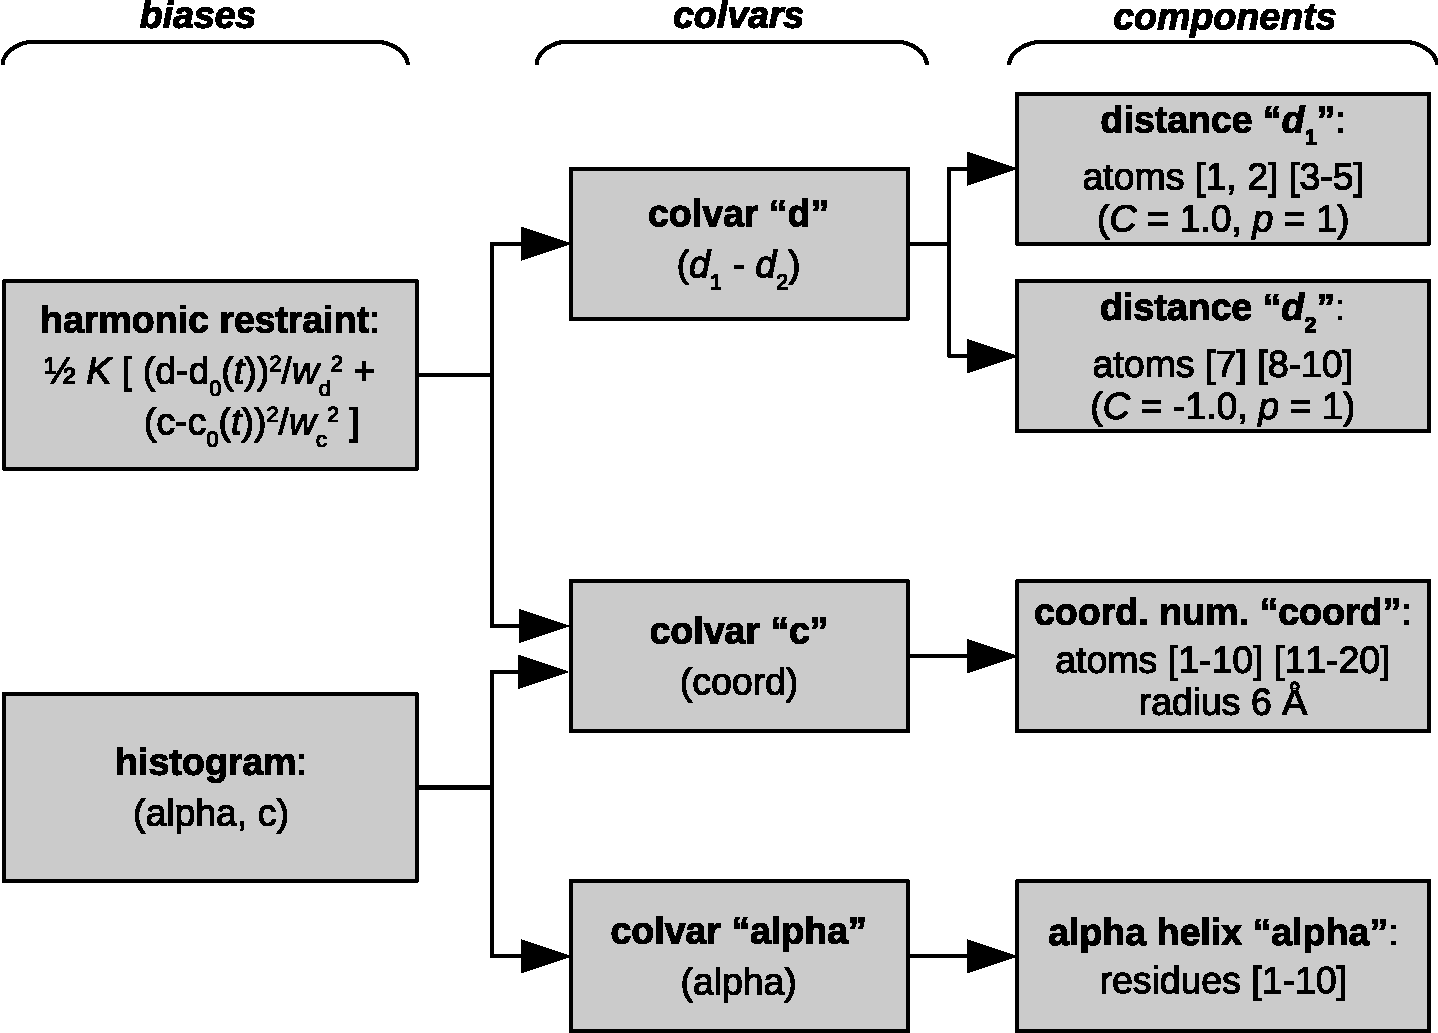
\includegraphics[width=12cm]{figures/colvars_diagram}
\else
  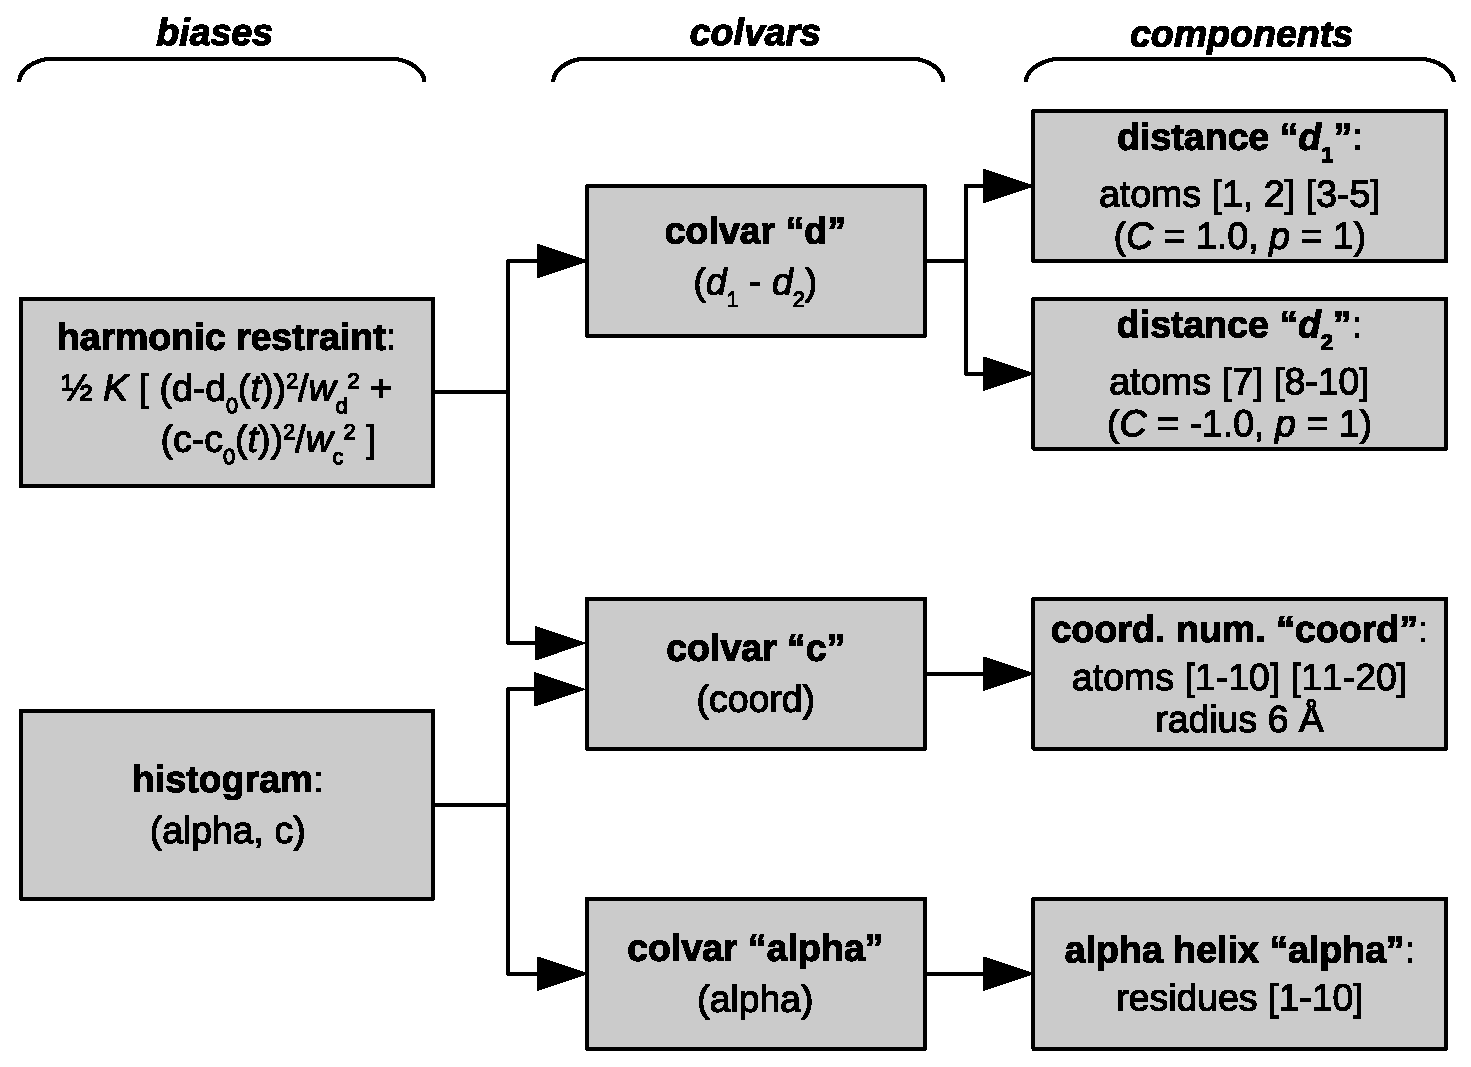
\includegraphics[width=12cm]{colvars_diagram}
\fi
  \caption{Graphical representation of a collective variables configuration.
    The colvar called ``$d$'' is defined as the difference between two distances: the first distance ($d_{1}$) is taken between the center of mass of atoms 1 and 2 and that of atoms 3 to 5, the second ($d_{2}$) between atom 7 and the center of mass of atoms 8 to 10.
The difference $d = d_{1} - d_{2}$ is obtained by multiplying the two by a coefficient $C = +1$ or $C = -1$, respectively.
The colvar called ``$c$'' is the coordination number calculated between atoms 1 to 10 and atoms 11 to 20.  A harmonic restraint is applied to both $d$ and $c$: to allow using the same force constant $K$, both $d$ and $c$ are scaled by their respective fluctuation widths $w_d$ and $w_c$.
A third colvar ``alpha'' is defined as the $\alpha$-helical content of residues 1 to 10.
The values of ``$c$'' and ``alpha'' are also recorded throughout the simulation as a joint 2-dimensional histogram.
\ifdefined\LAMMPS
\textbf{Note:} \emph{currently, the $\alpha$-helical content colvar is unavailable in LAMMPS, as it requires a name-based topology; future releases will overcome this limitation.}
\fi
}
  \label{fig:colvars_diagram}
\end{figure}


\ifdefined\NAMDCONF
\subsection{General parameters and input/output files}
\else
\section{General parameters and input/output files}
\fi
\label{sec:colvarmodule}

\ifdefined\NAMD
To enable a collective variable calculation, one or more parameters are added to the NAMD configuration file.
In \ref{sec:colvars_namd}, we document the syntax of such parameters.
One of these is the name of a configuration file for the collective variables module itself, which is described in \ref{sec:colvars_config}, and in the following sections.
\else\ifdefined\LAMMPS
To enable a collective variable calculation, one or more parameters are added to the LAMMPS configuration file.
In \ref{sec:colvars_lammps}, we document the syntax of such parameters.
\fi
\fi
One of these is the name of a configuration file for the collective variables module itself, which is described in \ref{sec:colvars_config}, and in the following sections.


\ifdefined\NAMD
\ifdefined\NAMDCONF
\subsubsection{NAMD parameters}
\else
\subsection{NAMD parameters}
\fi
\label{sec:colvars_namd}

To enable a collective variables-based calculation, two parameters must be added to the NAMD configuration file, \texttt{colvars} and \texttt{colvarsConfig}.
An optional third parameter, \texttt{colvarsInput}, can be used to continue a previous simulation.

\begin{itemize}
%  \setlength{\itemsep}{0.4cm}

\item %
  \keydef{%
    colvars}{%
    NAMD configuration file}{%
    Enable the collective variables module}{%
    boolean}{%
    \texttt{off}}{%
    If this flag is on, the collective variables module within
    NAMD is enabled; the module requires a separate configuration
    file, to be provided with \texttt{colvarsConfig}.}

\item %
  \key{%
    colvarsConfig}{%
    NAMD configuration file}{%
    Configuration file for the collective variables}{%
    UNIX filename}{%
    This file contains the definition of all collective variables and
    their biasing or analysis methods.
    Parameters within the configuration file can be controlled from
    a NAMD config file using Tcl variables in the following way:

    {\ttfamily
    colvars on\\
    colvarsConfig colvars\_subst.tmp\\
    set myParameter someValue\\
    \# Parse template and create specific config file on the fly\\
    set infile [open colvars\_template.in r] \\
    set outfile [open colvars\_subst.tmp w+] \\
    puts \$outfile [subst [read \$infile]] \\
    close \$infile \\
    close \$outfile}

    In this example, the string \texttt{\$myParameter} will be replaced
    with the value \texttt{someValue} wherever it appears in the file
    \texttt{colvars\_template.in}. This value will then be read in by
    the colvars module when it parses its input.
}

\item %
  \key{%
    colvarsInput}{%
    NAMD configuration file}{%
    Input state file for the collective variables}{%
    UNIX filename}{%
    When continuing a previous simulation run, this file contains the current state of all collective variables and of their associated algorithms.
    It is written automatically at the end of any simulation with collective variables.}

\end{itemize}

\else\ifdefined\LAMMPS
\subsection{LAMMPS keywords}
\label{sec:colvars_lammps}

To enable a collective variables-based calculation, the following line must be added to the LAMMPS configuration file:\\
\\
\texttt{fix } \emph{ID } \emph{group-ID }  \texttt{colvars } \emph{configfile } \emph{keyword values ...}\\
\\
where \emph{ID} and \emph{group-ID} are general options of the \texttt{fix} command, \emph{configfile} is the name of the configuration file for the collective variables module, and \emph{keyword} is one of the following optional keywords:

\begin{itemize}

\item %
  \key{%
    input}{%
    Keyword of the \texttt{fix colvars} command}{%
    Name or prefix of the input state file}{%
    string}{%
    If a value is provided, it is interpreted as either the name of the input state file, or as the prefix of the file named \emph{input}\texttt{.colvars.state}.
This allows to continue a previous collective variables-based calculation (see \ref{sec:colvars_input}).}

\item %
  \keydef{%
    output}{%
    Keyword of the \texttt{fix colvars} command}{%
    Prefix of the output state file}{%
    string}{%
    ``out''}{%
    If a value is provided, it is interpreted as the prefix to all output files that will be written by the collective variables module (see \ref{sec:colvars_output}).}

\item %
  \keydef{%
    unwrap}{%
    keyword of the \texttt{fix colvars} command}{%
    Whether to unwrap coordinates passed to the colvars module}{%
    ``yes'' or ``no''}{%
    ``yes''}{%
    This keyword controls whether wrapped or unwrapped coordinates are passed to the colvars module for     calculation of the collective variables and of the resulting forces.
The default is to use the image flags to reconstruct the absolute atom positions: under this convention, centers of mass and centers of geometry are calculated as a weighted vector sum (see \ref{sec:colvar_atom_groups_wrapping}).
Setting this to no will use the current local coordinates that are wrapped back into the simulation cell at each re-neighboring instead.}

\item %
  \keydef{%
    seed}{%
    Keyword of the \texttt{fix colvars} command}{%
    Seed for the random number generator}{%
    positive integer}{%
    1966}{%
    If defined, the value of this keyword is provided as seed to the random number generator.
    This is only meaningful when the \texttt{extendedLangevinDamping} keyword is used (see \ref{sec:colvar_extended}).}

\item %
  \keydef{%
    tstat}{%
    Keyword of the \texttt{fix colvars} command}{%
    Thermostating fix}{%
    string}{%
    NULL}{%
    This keyword provides the label of a thermostating fix that thermostats all atoms in the fix colvars group. This will be used to provide the colvars module with the current thermostat target temperature.}

\end{itemize}

\fi
\fi


\ifdefined\NAMDCONF
\subsubsection{Configuration file for the collective variables module}
\else
\subsection{Configuration file for the collective variables module}
\fi
\label{sec:colvars_config}

\ifdefined\NAMD
All the parameters defining the colvars and their biasing or analysis algorithms are read from the file
specified by \texttt{colvarsConfig}.
Hence, none of the keywords described in this section and the following ones are available as keywords for the
NAMD configuration file.
The syntax of the colvars configuration file is similar to that of the NAMD file
\ifdefined\NAMDCONF
 (see \ref{section:configsyntax})
\fi
, with a few important notes:
\else
The syntax of the colvars configuration file is ``\texttt{keyword value}'', where the keyword and its value are separated by any white space.
The following rules apply:
\fi

\begin{itemize}

\item keywords are case-insensitive (\texttt{upperBoundary} is the same as \texttt{upperboundary} and \texttt{UPPERBOUNDARY}): their string values are however case-sensitive (e.g.~file names);

\item a long value or a list of multiple values can be distributed across multiple lines by using curly braces, ``\texttt{\{}'' and ``\texttt{\}}'': the opening brace ``\texttt{\{}'' must occur on the same line as the keyword, following a space character or other white space; the closing brace ``\texttt{\}}'' can be at any position after that;

\ifdefined\NAMDCONF
\item many keywords are nested, and are only meaningful within a specific context: for every keyword documented in the following, the ``parent'' keyword that defines such context is also indicated in parentheses;
\else
\item many keywords are nested, and are only meaningful within a specific context: for every keyword documented in the following, the ``parent'' keyword that defines such context is also indicated;
\fi

\ifdefined\NAMD
\item unlike in the NAMD main configuration file, the deprecated `\texttt{=}' sign between a keyword and its value is not allowed;

\item unlike in the NAMD main configuration file,  Tcl commands and variables are not available, but it is possible to use Tcl to generate a new configuration file with different parameters
\ifdefined\NAMDCONF
(see \ref{sec:colvar_namd_parameters})
\fi
;
\fi

\item if a keyword requiring a boolean value (\texttt{yes|on|true} or \texttt{no|off|false}) is provided without an explicit value, it defaults to `\texttt{yes|on|true}'; for example, `\texttt{outputAppliedForce}' may be used as shorthand for `\texttt{outputAppliedForce on}';

\item the hash character \texttt{\#} indicates a comment: all text in the same line following this character will be ignored.

\end{itemize}

All parameters defining the colvars and their biasing or analysis algorithms are read from the file specified by \texttt{colvarsConfig}.
The following keywords are available in the global context of this configuration file, i.e.~not nested inside other keywords:
\begin{itemize}

\item %
  \keydef{%
    colvarsTrajFrequency}{%
    global}{%
  Colvar value trajectory frequency}{%
    positive integer}{%
    \texttt{100}}{%
    Thevalues of each colvar (and of other related quantities, if requested) are written to the file \outputName\texttt{.colvars.traj} every these many steps throughout the simulation.
    If the value is \texttt{0}, such trajectory file is not written.
    For optimization the output is buffered, and synchronized with the disk only when the restart file is being written.}

\item %
  \keydef{%
    colvarsTrajAppend}{%
    global}{%
    Append to trajectory file?}{%
    boolean}{%
    \texttt{off}}{%
    If this flag is enabled, and a file with the same name as the trajectory file is already present, new data is appended to that file.
    Otherwise, a new file is created with the same name that overwrites the previous file.
    \ifdefined\NAMD
\textbf{Note:} \emph{when
      running consecutive simulations with the same
    \outputName{} (e.g.~in FEP calculations), you should
      enable this option to preserve the previous contents of the
      trajectory file}.
\fi}

\item %
  \keydef{%
    colvarsRestartFrequency}{%
    global}{%
    Colvar module restart frequency}{%
    positive integer}{%
    \texttt{restartFreq}}{%
    Allows to choose a different restart frequency for the collective
    variables module.  Redefining it may be useful to trace the time
    evolution of those few properties which are not written to the
    trajectory file for reasons of disk space.}

\item %
  \key{%
    indexFile}{%
    global}{%
    Index file for atom selection (GROMACS ``ndx'' format)}{%
    UNIX filename}{%
    This option reads an index file (usually with a \texttt{.ndx}
    extension) as produced by the \texttt{make\_ndx} tool of GROMACS.
    \ifdefined\LAMMPS
    In LAMMPS, the \texttt{group2ndx} command can be used to generate such file from existing groups.
    \fi
    The names of index groups contained in this file can then be used to define
    atom groups with the \texttt{indexGroup} keyword.
    Other supported methods to select atoms are described in \ref{sec:colvar_atom_groups}.
  }

\item %
  \keydef{%
    analysis}{%
    global}{%
    Turn on run-time statistical analysis }{%
    boolean}{%
    \texttt{off}}{%
    If this flag is enabled, each colvar is instructed to perform
    whatever run-time statistical analysis it is configured to, such as
    correlation functions, or running averages and standard deviations.
    See section~\ref{sec:colvar_acf} for details.}

\end{itemize}

The example below defines the same configuration shown in Fig.~\ref{fig:colvars_diagram}.  The options within the \texttt{colvar} blocks are described in \ref{sec:colvar} and \ref{sec:cvc}, the ones within the \texttt{harmonic} and \texttt{histogram} blocks in \ref{sec:colvarbias}.
\textbf{Note:} \emph{except }\texttt{colvar}\emph{, none of the keywords shown is mandatory}.
\begin{verbatim}
colvar {
  # difference of two distances
  name d 
  width 0.2  # 0.2 Å of estimated fluctuation width 
  distance {
    componentCoeff  1.0
    group1 { atomNumbers 1 2 }
    group2 { atomNumbers 3 4 5 }
  }
  distance {
    componentCoeff -1.0
    group1 { atomNumbers 7 }
    group2 { atomNumbers 8 9 10 }
  }
}

colvar {
  name c
  coordNum {
    cutoff 6.0
    group1 { atomNumbersRange  1-10 }
    group2 { atomNumbersRange 11-20 }
  }
}
\end{verbatim}
\ifdefined\LAMMPS
\else
\begin{verbatim}
colvar {
  name alpha
  alpha {
    psfSegID PROT
    residueRange 1-10
  }
}
\end{verbatim}
\fi
\begin{verbatim}
harmonic {
  colvars d c
  centers 3.0 4.0
  forceConstant 5.0
}
\end{verbatim}
\ifdefined\LAMMPS
\begin{verbatim}
histogram {
  colvars c 
}
\end{verbatim}
\else
\begin{verbatim}
histogram {
  colvars c alpha
}
\end{verbatim}
\fi

Section \ref{sec:colvar} explains how to define a colvar and its behavior, regardless of its specific functional form.
To define colvars that are appropriate to a specific physical system, Section \ref{sec:colvar_atom_groups} documents how to select atoms, and section \ref{sec:cvc} lists all of the available functional forms, which we call ``colvar components''.
Finally, section \ref{sec:colvarbias} lists the available methods and algorithms to perform biased simulations and multidimensional analysis of colvars.


\ifdefined\NAMDCONF
\subsubsection{Input state file (optional)}
\else
\subsection{Input state file (optional)}
\fi
\label{sec:colvars_input}

Aside from the configuration file, an optional input state file may be provided to continue a previous simulation.
\ifdefined\NAMD
The name of this file is provided as a value to the keyword \texttt{colvarsInput}.
\else\ifdefined\LAMMPS
The name of this file is provided as the argument to the \texttt{input} keyword of the \texttt{fix ID group-ID colvars} command.
\fi
\fi


\ifdefined\NAMDCONF
\subsubsection{Output files}
\else
\subsection{Output files}
\fi
\label{sec:colvars_output}

\ifdefined\NAMD
In addition to the NAMD output files, the following three output files are written:
\else
In addition to the output files written by the MD program, the following three output files are written:
\fi

\begin{itemize}

\item a \emph{state file}, named \outputName\texttt{.colvars.state}; this file is in ASCII format%
\ifdefined\NAMD%
, regardless of the value of \texttt{binaryOutput} in the NAMD configuration; to continue the simulation, the name of this file must be included in the configuration of the next run using \texttt{colvarsInput}, together with the other NAMD output files;
\else%
.
\fi

\ifdefined\NAMD
\item if the NAMD parameter \texttt{restartFreq} is larger than zero, a \emph{restart file} named\\ \restartName\texttt{.colvars.state} is written, which is equivalent to the state file; the frequency of writing is every \texttt{restartFreq} steps, or every \texttt{colvarsRestartFrequency} steps if defined; 
\else
\item if the parameter \texttt{colvarsRestartFrequency} is larger than zero, a \emph{restart file} named\\ \restartName\texttt{.colvars.state} is written, which is equivalent to the state file; 
\fi

\item if the parameter \texttt{colvarsTrajFrequency} is greater than 0 (default: 100), a \emph{trajectory file} is written during the simulation: its name is \outputName\texttt{.colvars.traj}; unlike the state file, it is not needed to restart a simulation, but can be used later for post-processing and analysis.

\end{itemize}

Other output files may be written by specific methods applied to the colvars (e.g.~by the ABF method, see \ref{sec:colvarbias_abf}, or the metadynamics method, see \ref{sec:colvarbias_meta}).
Like the colvar trajectory file, they are needed only for analyzing, not continuing a simulation.
All such files' names also begin with the prefix \outputName\texttt{}.

\ifdefined\NAMD
Finally, the total energy of all biases or restraints applied to the colvars appears under the NAMD standard output, under the MISC column.
\fi


\ifdefined\NAMDCONF
\subsection{Defining collective variables and their properties}
\else
\section{Defining collective variables and their properties}
\fi
\label{sec:colvar}

In the configuration file each colvar is defined by the keyword
\texttt{colvar}, followed by its configuration options within curly braces: \texttt{colvar~\{~...~\}}.  One of these options is the name of a colvar component: for example, including \texttt{rmsd \{~...~\}} defines the colvar as a RMSD function.  \emph{In most applications, only one component is used, and the component is equal to the colvar.}

The full list of colvar components can be found in Section~\ref{sec:cvc}, with the syntax to select atoms in Section~\ref{sec:colvar_atom_groups}. 
The following section lists several options to control the behavior of a single colvar, regardless of its type.

\ifdefined\NAMDCONF
\subsubsection{General options for a collective variable}
\else
\subsection{General options for a collective variable}
\fi
\label{sec:colvar_general}
The following options are not required by default; however, the first four are very  frequently used:
\begin{itemize}

\item %
  \keydef{%
    name}{%
    \texttt{colvar}}{%
    Name of this colvar}{%
    string}{%
    ``\texttt{colvar}'' + numeric id}{%
    The name is an unique case-sensitive string which allows the
    colvar module to identify this colvar unambiguously; it is also
    used in the trajectory file to label to the columns corresponding
    to this colvar.}

\item %
  \keydef{%
    width}{%
    \texttt{colvar}}{%
    Expected fluctuations amplitude, and resolution for grid-based methods}{%
    positive decimal}{%
    1.0}{%
    This number is a user-provided estimate of the fluctuation amplitude for the colvar.  For example, it is recommended to set this number smaller than or equal to the standard deviation of the colvar during a very short simulation run.  Biasing algorithms use this parameter for different purposes:
    harmonic restraints (\ref{sec:colvarbias_harmonic}) use it to set the physical unit of the force constant, the histogram
    (\ref{sec:colvarbias_histogram}) and ABF biases
    (\ref{sec:colvarbias_abf}) interpret it as the grid spacing in the
    direction of this variable, and metadynamics
    (\ref{sec:colvarbias_meta}) uses it to set the width of newly
    added hills.  This number is expressed in the same physical unit
    as the colvar value.}

\item %
  \key{%
    lowerBoundary}{%
    \texttt{colvar}}{%
    Lower boundary of the colvar}{%
    decimal}{%
    Defines the lowest end of the interval of ``relevant'' values for the colvar.
    This number can be either a true physical boundary, or a user-defined number.  
    Together with \texttt{upperBoundary} and \texttt{width}, it is used to define a grid of values along the colvar (not available for colvars based on \texttt{distanceDir}, \texttt{distanceVec}, and \texttt{orientation}).
    This option does not affect dynamics: to confine a colvar within a certain interval, the options \texttt{lowerWall} and \texttt{lowerWallConstant} should be used.
}

\item %
  \key{%
    upperBoundary}{%
    \texttt{colvar}}{%
    Upper boundary of the colvar}{%
    decimal}{%
    Similarly to \texttt{lowerBoundary}, defines the highest possible or allowed value.}

\item %
  \keydef{%
    hardLowerBoundary}{%
    \texttt{colvar}}{%
    Whether the lower boundary is the physical lower limit}{%
    boolean}{%
    \texttt{off}}{%
    This option does not affect simulation results, but enables some internal optimizations.
    Depending on its mathematical definition, a colvar may have ``natural'' boundaries: for example, a \texttt{distance} colvar has a ``natural'' lower boundary at 0~\AA.  Setting this option instructs the colvars module that the user-defined lower boundary is ``natural''.
See Section~\ref{sec:cvc} for the physical ranges of values of each component.}

\item %
  \keydef{%
    hardUpperBoundary}{%
    \texttt{colvar}}{%
    Whether the upper boundary is the physical upper limit of the colvar's values}{%
    boolean}{%
    \texttt{off}}{%
    Analogous to \texttt{hardLowerBoundary}.}

\item %
  \keydef{%
    expandBoundaries}{%
    \texttt{colvar}}{%
    Allow to expand the two boundaries if needed}{%
    boolean}{%
    \texttt{off}}{%
    If defined, biasing and analysis methods may keep their own copies
    of \texttt{lowerBoundary} and \texttt{upperBoundary}, and expand
    them to accommodate values that do not fit in the initial range.
    Currently, this option is used by the metadynamics bias
    (\ref{sec:colvarbias_meta}) to keep all of its hills fully within
    the grid.  This option cannot be used when
      the initial boundaries already span the full period of a periodic
      colvar.}
\end{itemize}


\ifdefined\NAMDCONF
\paragraph*{Artificial boundary potentials (walls)}
\else
\subsection{Artificial boundary potentials (walls)}
\fi
The following options are useful to define restraints (confining potentials) for this colvar.
To apply moving restraints, or restraints to more than one colvar simultaneously, a more convenient option is to use the \texttt{harmonic} bias (\ref{sec:colvarbias_harmonic}).

\begin{itemize}

\item %
  \key{%
    lowerWallConstant}{%
    \texttt{colvar}}{%
    Lower wall force constant (kcal/mol)}{%
    positive decimal}{%
    Defines the force constant for a confining restraint on the colvar, in the form of a     ``half-harmonic'' potential.
    The potential starts at \texttt{lowerWall} if it is defined, or     \texttt{lowerBoundary} otherwise.
    The energy unit of the constant is kcal/mol, while the spatial unit is that of the colvar.}

\item %
  \keydef{%
    lowerWall}{%
    \texttt{colvar}}{%
    Position of the lower wall}{%
    decimal}{%
    \texttt{lowerBoundary}}{%
    Defines the value below which a confining restraint on the colvar is applied, in the form of a ``half-harmonic'' potential.
    Allows to use a different position of the wall than \texttt{lowerBoundary}.}

\item %
  \key{%
    upperWallConstant}{%
    \texttt{colvar}}{%
    Upper wall force constant (kcal/mol)}{%
    positive decimal}{%
    Analogous to \texttt{lowerWallConstant}.}

\item %
  \keydef{%
    upperWall}{%
    \texttt{colvar}}{%
    Position of the upper wall}{%
    decimal}{%
    \texttt{upperBoundary}}{%
    Analogous to \texttt{lowerWall}.}
\end{itemize}


\ifdefined\NAMDCONF
\paragraph*{Trajectory output}
\else
\subsection{Trajectory output}
\fi
\begin{itemize}
\item %
  \keydef{%
    outputValue}{%
    \texttt{colvar}}{%
    Output a trajectory for this colvar}{%
    boolean}{%
    \texttt{on}}{%
    If \texttt{colvarsTrajFrequency} is non-zero, the value of this
    colvar is written to the trajectory file every
    \texttt{colvarsTrajFrequency} steps in the column labeled
    ``$<$\texttt{name}$>$''.}

\item %
  \keydef{%
    outputVelocity}{%
    \texttt{colvar}}{%
    Output a velocity trajectory for this colvar}{%
    boolean}{%
    \texttt{off}}{%
    If \texttt{colvarsTrajFrequency} is defined, the
    finite-difference calculated velocity of this colvar are written
    to the trajectory file under the label
    ``\texttt{v\_}$<$\texttt{name}$>$''.}

\item %
  \keydef{%
    outputEnergy}{%
    \texttt{colvar}}{%
    Output an energy trajectory for this colvar}{%
    boolean}{%
    \texttt{off}}{%
    This option applies only to extended Lagrangian colvars. If
    \texttt{colvarsTrajFrequency} is defined, the kinetic energy of
    the extended degree and freedom and the potential energy of the
    restraining spring are are written to the trajectory file under
    the labels ``\texttt{Ek\_}$<$\texttt{name}$>$'' and
    ``\texttt{Ep\_}$<$\texttt{name}$>$''.}

\item %
  \keydef{%
    outputSystemForce}{%
    \texttt{colvar}}{%
    Output a system force trajectory for this
    colvar}{%
    boolean}{%
    \texttt{off}}{%
    If \texttt{colvarsTrajFrequency} is defined, the total system force on this
    colvar (i.e.~the projection of all interatomic forces
    except constraint forces on this colvar --- see
    equation~(\ref{eq:gradient_vector}) in
    section~\ref{sec:colvarbias_abf}) are written to the trajectory
    file under the label ``\texttt{fs\_}$<$\texttt{name}$>$''.  \textbf{Note:} not all components support this option.  The
    physical unit for this force is kcal/mol divided by the colvar
    unit.}

\item %
  \keydef{%
    outputAppliedForce}{%
    \texttt{colvar}}{%
    Output an applied force trajectory for this
    colvar}{%
    boolean}{%
    \texttt{off}}{%
    If \texttt{colvarsTrajFrequency} is defined, the total force
    applied on this colvar by biases within the colvar module are
    written to the trajectory under the label
    ``\texttt{fa\_}$<$\texttt{name}$>$''.  The physical unit for this
    force is kcal/mol divided by the colvar unit.}
\end{itemize}


\ifdefined\NAMDCONF
\paragraph*{Extended Lagrangian.}
\else
\subsection{Extended Lagrangian.}
\fi
\label{sec:colvar_extended}

The following options enable extended-system
dynamics, where a colvar is coupled to an additional degree of freedom 
(fictitious particle) by a harmonic spring.

\begin{itemize}
\item %
  \keydef{%
    extendedLagrangian}{%
    \texttt{colvar}}{%
    Add extended degree of freedom}{%
    boolean}{%
    \texttt{off}}{%
    Adds a fictitious particle to be coupled to the colvar by a harmonic
    spring. The fictitious mass and the force constant of the coupling
    potential are derived from the parameters \texttt{extendedTimeConstant}
    and \texttt{extendedFluctuation}, described below. Biasing forces on the
    colvar are applied to this fictitious particle, rather than to the
    atoms directly.  This implements the extended Lagrangian formalism
    used in some metadynamics simulations~\cite{Iannuzzi2003}.
    \ifdefined\NAMD
    The energy associated with the extended degree of freedom is reported
    under the MISC title in NAMD's energy output.
    \fi
    }

\item %
  \keydef{%
    extendedFluctuation}{%
    \texttt{colvar}}{%
    Standard deviation between the colvar and the fictitious
    particle (colvar unit)}{%
    positive decimal}{%
    \texttt{width}}{%
    Defines the spring stiffness for the \texttt{extendedLagrangian}
    mode, by setting the typical deviation between the colvar and the extended
    degree of freedom due to thermal fluctuation.
    The spring force constant is calculated internally as $k_B T / \sigma^2$,
    where $\sigma$ is the value of \texttt{extendedFluctuation}.}

\item %
  \keydef{%
    extendedTimeConstant}{%
    \texttt{colvar}}{%
    Oscillation period of the fictitious particle (fs)}{%
    positive decimal}{%
    \texttt{200}}{%
    Defines the inertial mass of the fictitious particle, by setting the
    oscillation period of the harmonic oscillator formed by the fictitious
    particle and the spring. The period
    should be much larger than the MD time step to ensure accurate integration
    of the extended particle's equation of motion.
    The fictitious mass is calculated internally as $k_B T (\tau/2 \pi \sigma)^2$,
    where $\tau$ is the period and $\sigma$ is the typical fluctuation (see above).}

\item %
  \keydef{%
    extendedTemp}{%
    \texttt{colvar}}{%
    Temperature for the extended degree of freedom (K)}{%
    positive decimal}{%
    thermostat temperature}{%
    Temperature used for calculating the coupling force constant of the
    extended coordinate (see \texttt{extendedFluctuation}) and, if needed, as a
    target temperature for extended Langevin dynamics (see
    \texttt{extendedLangevinDamping}). This should normally be left at its
    default value.}

\item %
  \keydef{%
    extendedLangevinDamping}{%
    \texttt{colvar}}{%
    Damping factor for extended Langevin dynamics
    (ps$^{-1}$)}{%
    positive decimal}{%
    \texttt{1.0}}{%
    If this is non-zero, the extended degree of freedom undergoes Langevin dynamics
    at temperature \texttt{extendedTemp}. The friction force is minus
    \texttt{extendedLangevinDamping} times the velocity. This is useful because
    the extended dynamics coordinate may heat up in the transient
    non-equilibrium regime of ABF. Use moderate damping values, to limit
    viscous friction (potentially slowing down diffusive sampling) and stochastic
    noise (increasing the variance of statistical measurements). In
    doubt, use the default value.}
\end{itemize}


\ifdefined\NAMDCONF
\subsubsection{Statistical analysis of collective variables}
\else
\subsection{Statistical analysis of collective variables}
\fi
\label{sec:colvar_acf}

When the global keyword \texttt{analysis} is defined in the
configuration file, run-time calculations of statistical properties for
individual colvars can be performed.  At the moment, several types of
time correlation functions, running averages and running standard
deviations are available.

\begin{itemize}

\item %
  \keydef{%
    corrFunc}{%
    \texttt{colvar}}{%
    Calculate a time correlation function?}{%
    boolean}{%
    \texttt{off}}{%
    Whether or not a time correlaction function should be calculated
    for this colvar.}

\item %
  \key{%
    corrFuncWithColvar}{%
    \texttt{colvar}}{%
    Colvar name for the correlation function}{%
    string}{%
    By default, the auto-correlation function (ACF) of this colvar,
    $\xi_{i}$, is calculated.  When this option is specified, the
    correlation function is calculated instead with another colvar,
    $\xi_{j}$, which must be of the same type (scalar, vector, or
    quaternion) as $\xi_{i}$.}

\item%
  \keydef{%
    corrFuncType}{%
    \texttt{colvar}}{%
    Type of the correlation function}{%
    \texttt{velocity}, \texttt{coordinate} or
    \texttt{coordinate\_p2}}{%
    \texttt{velocity}}{%
    With \texttt{coordinate} or \texttt{velocity}, the correlation
    function $C_{i,j}(t)$~= $\left\langle \Pi\left(\xi_{i}(t_{0}),
        \xi_{j}(t_{0}+t)\right) \right\rangle$ is calculated between
    the variables $\xi_{i}$ and $\xi_{j}$, or their velocities.
    $\Pi(\xi_{i}, \xi_{j})$ is the scalar product when calculated
    between scalar or vector values, whereas for quaternions it is the
    cosine between the two corresponding rotation axes.  With
    \texttt{coordinate\_p2}, the second order Legendre polynomial,
    $(3\cos(\theta)^{2}-1)/2$, is used instead of the cosine.}

\item %
  \keydef{%
    corrFuncNormalize}{%
    \texttt{colvar}}{%
    Normalize the time correlation function?}{%
    boolean}{%
    \texttt{on}}{%
    If enabled, the value of the correlation function at $t$~= 0
    is normalized to 1; otherwise, it equals to $\left\langle
      O\left(\xi_{i}, \xi_{j}\right) \right\rangle$.}

\item %
  \keydef{%
    corrFuncLength}{%
    \texttt{colvar}}{%
    Length of the time correlation function}{%
    positive integer}{%
    \texttt{1000}}{%
    Length (in number of points) of the time correlation function.}

\item %
  \keydef{%
    corrFuncStride}{%
    \texttt{colvar}}{%
    Stride of the time correlation function}{%
    positive integer}{%
    \texttt{1}}{%
    Number of steps between two values of the time correlation function.}

\item %
  \keydef{%
    corrFuncOffset}{%
    \texttt{colvar}}{%
    Offset of the time correlation function}{%
    positive integer}{%
    \texttt{0}}{%
    The starting time (in number of steps) of the time correlation
    function (default: $t$~= 0).  \textbf{Note:} \emph{the value at $t$~= 0 is always
    used for the normalization}.}

\item %
  \keydef{%
    corrFuncOutputFile}{%
    \texttt{colvar}}{%
    Output file for the time correlation function}{%
    UNIX filename}{%
    \texttt{$<$name$>$.corrfunc.dat}}{%
    The time correlation function is saved in this file.}

\item %
  \keydef{%
    runAve}{%
    \texttt{colvar}}{%
    Calculate the running average and standard deviation}{%
    boolean}{%
    \texttt{off}}{%
    Whether or not the running average and standard deviation should
    be calculated for this colvar.}

\item %
  \keydef{%
    runAveLength}{%
    \texttt{colvar}}{%
    Length of the running average window}{%
    positive integer}{%
    \texttt{1000}}{%
    Length (in number of points) of the running average window.}

\item %
  \keydef{%
    runAveStride}{%
    \texttt{colvar}}{%
    Stride of the running average window values}{%
    positive integer}{%
    \texttt{1}}{%
    Number of steps between two values within the running average window.}

\item %
  \keydef{%
    runAveOutputFile}{%
    \texttt{colvar}}{%
    Output file for the running average and standard deviation}{%
    UNIX filename}{%
    \texttt{$<$name$>$.runave.dat}}{%
    The running average and standard deviation are saved in this file.}

\end{itemize}



\ifdefined\NAMDCONF
\subsubsection{Selecting atoms for colvars: defining atom groups}
\label{sec:colvar_atom_groups}
\else
\section{Selecting atoms for colvars: defining atom groups}
\label{sec:colvar_atom_groups}

\subsection{Selection keywords}
\fi
\label{sec:colvar_atom_groups_sel}

To define collective variables, atoms are usually selected by group.  Each group is identified by a name that is unique in the context of the specific colvar component (e.g.~for a distance component, the names of the two groups are \texttt{group1} and \texttt{group2}).
The name is followed by a brace-delimited block of selection keywords: these may be used individually or in combination with each other, and each can be repeated any number of times.
Selection is incremental: each keyword adds the corresponding atoms to the selection, so that different sets of atoms can be combined.
However, atoms included by multiple keywords are only counted once.
Below is a example configuration for an atom group with name ``\texttt{atoms}'', which uses an unusually varied combination of selection keywords:
\begin{verbatim}
atoms {

  # add atoms 1 and 3 to this group (note: the first atom in the system is 1)
  atomNumbers { 
    1 3
  }
\end{verbatim}
\ifdefined\NAMD
\begin{verbatim}
  # add all the atoms with occupancy 2 in the file atoms.pdb
  atomsFile             atoms.pdb
  atomsCol              O
  atomsColValue         2.0

  # add all the C-alphas within residues 11 to 20 of segments "PR1" and "PR2"
  psfSegID              PR1 PR2
  atomNameResidueRange  CA 11-20
  atomNameResidueRange  CA 11-20
\end{verbatim}
\else
\begin{verbatim}
  # add atoms starting from 20 up to and including 50
  atomNumbersRange  20-50

  # add index group (requires a .ndx file to be provided globally)
  indexGroup Water
\end{verbatim}
\fi
\begin{verbatim}
}
\end{verbatim}
\ifdefined\NAMD
The resulting selection includes atoms 1 and 3, those indicated by a flag in the given PDB file, as well as theC$_\alpha$ atoms selected by name, segment, and residue numbers. 
\else
The resulting selection includes atoms 1 and 3, those between 20 and 50, and those in the index group called ``Water''; the indices of this group are read from the file provided by \texttt{indexFile}, in the global section of the configuration file.
\fi
\\

The list of selection keywords is:

\begin{itemize}

\item %
  \key{%
    atomNumbers}{%
    atom group}{%
    List of atom numbers}{%
    space-separated list of positive integers}{%
    This option adds to the group all the atoms whose numbers are in
    the list.  \emph{The number of the first atom in the system is 1: to convert from a VMD selection, use ``atomselect get serial''.}
  }


\item %
  \key{%
    indexGroup}{%
    atom group}{%
    Name of index group to be used (GROMACS format)}{%
    string}{%
    If the name of an index file has been provided by \texttt{indexFile}, this option allows to select one index group from that file: the atoms from that index group will be used to define the current group.}

\item %
  \key{%
    atomNumbersRange}{%
    atom group}{%
    Atoms within a number range}{%
    $<$Starting number$>$-$<$Ending number$>$}{%
    This option includes in the group all atoms whose numbers are within the range specified.  \emph{The number of the first atom in the system is 1.}
  }

\ifdefined\LAMMPS
\else
\item %
  \key{%
    atomNameResidueRange}{%
    atom group}{%
    Named atoms within a range of residue numbers}{%
    $<$Atom name$>$ $<$Starting residue$>$-$<$Ending residue$>$}{%
    This option adds to the group all the atoms with the provided
    name, within residues in the given range.}

\item %
  \key{%
    psfSegID}{%
    atom group}{%
    PSF segment identifier}{%
    space-separated list of strings (max 4 characters)}{%
    This option sets the PSF segment identifier for
    \texttt{atomNameResidueRange}.  Multiple values may be provided,
    which correspond to multiple instances of
    \texttt{atomNameResidueRange}, in the order of their occurrence.
    This option is only necessary if a PSF topology file is used.}

\item %
  \key{%
    atomsFile}{%
    atom group}{%
    PDB file name for atom selection}{%
    UNIX filename}{%
    This option selects atoms from the PDB file provided and adds them
    to the group according to numerical flags in the column
    \texttt{atomsCol}.  \textbf{Note:} \emph{the sequence of atoms in the PDB file
    provided must match that in the system's topology}.}

\item %
  \key{%
    atomsCol}{%
    atom group}{%
    PDB column to use for atom selection flags}{%
    \texttt{O}, \texttt{B}, \texttt{X}, \texttt{Y}, or \texttt{Z}}{%
    This option specifies which PDB column in \texttt{atomsFile} is used to determine which atoms are to be included in the group.
  }

\item %
  \key{%
    atomsColValue}{%
    atom group}{%
    Atom selection flag in the PDB column}{%
    positive decimal}{%
    If defined, this value in \texttt{atomsCol} identifies atoms in \texttt{atomsFile} that are included in the group.
    If undefined, all atoms with a non-zero value in \texttt{atomsCol} are included.}
\fi

\item %
  \key{%
    dummyAtom}{%
    atom group}{%
    Dummy atom position (\AA{})}{%
    \texttt{(x, y, z)} triplet}{%
    Instead of selecting any atom, this option makes the group a virtual particle at a fixed position in space.  This is useful e.g.~to replace a group's center of geometry with a user-defined position.}

\end{itemize}

\ifdefined\NAMDCONF
\paragraph*{Moving frame of reference.} 
\else
\subsection{Moving frame of reference.} 
\fi
\label{sec:colvar_atom_groups_ref_frame}

The following options define an automatic calculation of an optimal translation (\texttt{centerReference}) or optimal rotation (\texttt{rotateReference}), that superimposes the positions of this group to a provided set of reference coordinates.
This can allow, for example, to effectively remove from certain colvars the effects of molecular tumbling and of diffusion.
Given the set of atomic positions $\mathbf{x}_{i}$, the colvar $\xi$ can be defined on a set of roto-translated positions $\mathbf{x}_{i}' = R(\mathbf{x}_{i} - \mathbf{x}^{\mathrm{C}}) + \mathbf{x}^{\mathrm{ref}}$.
$\mathbf{x}^{\mathrm{C}}$ is the geometric center of the $\mathbf{x}_{i}$, $R$ is the optimal rotation matrix to the reference positions and $\mathbf{x}^{\mathrm{ref}}$ is the geometric center of the reference positions.

Components that are defined based on pairwise distances are naturally invariant under global roto-translations.
Other components are instead affected by global rotations or translations: however, they can be made invariant if they are expressed in the frame of reference of a chosen group of atoms, using the \texttt{centerReference} and \texttt{rotateReference} options.
Finally, a few components are defined by convention using a roto-translated frame (e.g. the minimal RMSD): for these components, \texttt{centerReference} and \texttt{rotateReference} are enabled by default.
In typical applications, the default settings result in the expected behavior.


\begin{itemize}

\item %
  \keydef{%
    centerReference}{%
    atom group}{%
    Implicitly remove translations for this group}{%
    boolean}{%
    \texttt{off}}{%
    If this option is \texttt{on}, the center of geometry of the group will be aligned with that of the reference positions provided by%
\ifdefined\LAMMPS
 \texttt{refPositions}.
\else
 either \texttt{refPositions} or \texttt{refPositionsFile}.
\fi
    Colvar components will only have access to the aligned positions.
\textbf{Note}: unless otherwise specified, \texttt{rmsd} and \texttt{eigenvector} set this option to \texttt{on} \emph{by default}.
}

\item %
  \keydef{%
    rotateReference}{%
    atom group}{%
    Implicitly remove rotations for this group}{%
    boolean}{%
    \texttt{off}}{%
    If this option is \texttt{on}, the coordinates of this group will be optimally superimposed to the reference positions provided by%
\ifdefined\LAMMPS
\texttt{refPositions}.
\else
either \texttt{refPositions} or \texttt{refPositionsFile}.
\fi
    The rotation will be performed around the center of geometry if \texttt{centerReference} is \texttt{on}, around the origin otherwise.
    The algorithm used is the same employed by the \texttt{orientation} colvar component     \cite{Coutsias2004}.
    Forces applied to the atoms of this group will also be implicitly rotated back to the original frame.
    \textbf{Note}: unless otherwise specified, \texttt{rmsd} and \texttt{eigenvector} set this option to \texttt{on} \emph{by default}.
}

\item %
  \key{%
    refPositions}{%
    atom group}{%
    Reference positions for fitting (\AA)}{%
    space-separated list of \texttt{(x, y, z)} triplets}{%
    This option provides a list of reference coordinates for \texttt{centerReference} or \texttt{rotateReference}.
    If only \texttt{centerReference} is \texttt{on}, the list may contain a single (x, y, z) triplet; if also \texttt{rotateReference} is \texttt{on}, the list should be as long as the atom group.
}

\ifdefined\LAMMPS
\else
\item %
  \key{%
    refPositionsFile}{%
    atom group}{%
    File containing the reference positions for fitting}{%
    UNIX filename}{%
    Supplies the reference positions (mutually exclusive with \texttt{refPositions}).
    Atomic positions are read differently depending on the three following scenarios:
    \emph{i)} \texttt{refPositionsCol} is specified: the PDB file contains a set of position larger than the size of the group, and positions are read according to the value of the column \texttt{refPositionsCol} (which may be the same as \texttt{atomsCol}).
    \emph{ii)} \texttt{refPositionsCol} is not specified and the PDB file contains exactly as many \texttt{ATOM} records as the atoms in the group: all positions are read in sequence;
    \emph{iii)} \texttt{refPositionsCol} is not specified and the PDB file contains the entire system: the positions corresponding to the numeric indices of the atom group are read.
}

\item %
  \key{%
    refPositionsCol}{%
    atom group}{%
    PDB column containing atom flags}{%
    \texttt{O}, \texttt{B}, \texttt{X}, \texttt{Y}, or \texttt{Z}}{%
    Like \texttt{atomsCol} for \texttt{atomsFile}, indicates which column to use to identify the atoms in \texttt{refPositionsFile}.}

\item %
  \key{%
    refPositionsColValue}{%
    atom group}{%
    Atom selection flag in the PDB column}{%
    positive decimal}{%
    Analogous to \texttt{atomsColValue}, but applied to \texttt{refPositionsCol}.}
\fi
\item %
  \keydef{%
    refPositionsGroup}{%
    atom group}{%
    Use an alternate set of atoms to define the roto-translation}{%
    Block \texttt{refPositionsGroup \{ ... \}}}{%
    This group itself}{%
    If either \texttt{centerReference} or \texttt{rotateReference} is defined, this keyword defines an alternate atom group to calculate the optimal roto-translation.
    Use this option to define a continuous rotation if the structure of the group involved changes significantly (a typical symptom would be the message ``Warning: discontinuous rotation!'').

\ifdefined\LAMMPS
\else
    The following example illustrate the syntax of \texttt{refPositionsGroup}: a group called ``\texttt{atoms}''     is defined, including 8 C$_{\alpha}$ atoms of a protein of 100 residues.
    An optimal roto-translation is calculated automatically by fitting the C$_{\alpha}$ trace of the rest of the protein onto the coordinates provided by a PDB file.}
\begin{verbatim}
# Example: defining a group "atoms", with its coordinates expressed 
# on a roto-translated frame of reference defined by a second group
atoms {

  psfSegID              PROT
  atomNameResidueRange  CA 41-48

  centerReference yes
  rotateReference yes
  refPositionsGroup {
    # define the frame by fitting the rest of the protein
    psfSegID              PROT PROT
    atomNameResidueRange  CA  1-40
    atomNameResidueRange  CA 49-100
  } 
  refPositionsFile all.pdb  # can be the entire system
}
\end{verbatim}
\fi
\end{itemize}

The following two options have default values appropriate for the vast majority of applications, and are only provided to support rare, special cases.
\begin{itemize}

\item %
  \keydef{%
    enableFitGradients}{%
    atom group}{%
    Include the roto-translational contribution to colvar gradients}{%
    boolean}{%
    \texttt{on}}{%
    When either \texttt{centerReference} or \texttt{rotateReference} is on,
    the gradients of some colvars include terms proportional to
    $\partial{}R/\partial\mathbf{x}_{i}$ (rotational gradients) and
    $\partial\mathbf{x}^{\mathrm{C}}/\partial\mathbf{x}_{i}$ (translational gradients).
    By default, these terms are calculated and included in the total gradients;
    if this option is set to \texttt{off}, they are neglected.
}

\item %
  \keydef{%
    enableForces}{%
    atom group}{%
    Apply forces from this colvar to this group}{%
    boolean}{%
    \texttt{on}}{%
    If this option is \texttt{off}, no forces are applied from this
    colvar to this group. Other forces are not affected (i.e. those
    from the MD engine, from other colvars, and other external forces).
    For dummy atoms, this option is on by default.
 }

\end{itemize}


\ifdefined\NAMDCONF
\paragraph*{Treatment of periodic boundary conditions.}
\else
\subsection{Treatment of periodic boundary conditions.}
\fi
\label{sec:colvar_atom_groups_wrapping}

\ifdefined\NAMD
 In simulations with periodic boundary conditions, NAMD maintains
  the coordinates of all the atoms within a molecule contiguous to
  each other (i.e.~there are no spurious ``jumps'' in the molecular
  bonds).  The colvar module relies on this when calculating a group's
  center of geometry, but the condition may fail if the group spans
  different molecules: in that case, writing the NAMD output files
  \texttt{wrapAll} or \texttt{wrapWater} could produce wrong results
  when a simulation run is continued from a previous one.  
  The user should then determine, according to which
  type of colvars are being calculated, whether \texttt{wrapAll} or
  \texttt{wrapWater} can be enabled.
  In general, internal coordinate wrapping by NAMD does not affect the calculation of colvars if each atom group satisfies one or more of the following:
\else\ifdefined\LAMMPS
In simulations with periodic boundary conditions, many of the implemented colvar components rely on the fact that each position within a group of atoms is at the nearest periodic image from the center of geometry of the group itself.
However, due to the internal wrapping of individual atomic positions done by LAMMPS, this assumption is inaccurate if groups lies at one of the unit cell's boundaries.
For this reason, within the colvars module coordinates are unwrapped by default to avoid discontinuities due to coordinate wrapping (see \texttt{unwrap} keyword in \ref{sec:colvars_lammps}).
The user should determine whether maintaining the default value of \texttt{unwrap}, depending on the specifics of each system.
In general, internal coordinate wrapping by LAMMPS does not affect the calculation of colvars if each atom group satisfies one or more of the following:
\fi
% each code will need its own wrapping considerations.
\fi

\begin{enumerate}
  \item[\emph{i)}] it is composed by only one atom;
\ifdefined\NAMD
  \item[\emph{ii)}] it has all its atoms within the same molecule;
  \item[\emph{iii)}] %
\else
  \item[\emph{ii)}] %
\fi %
    it is used by a colvar component which does not make use of its center of geometry, but only of pairwise distances (\texttt{distanceInv}, \texttt{coordNum}, \texttt{hBond}, \texttt{alpha}, \texttt{dihedralPC});
\ifdefined\NAMD
  \item[\emph{iv)}] %
\else
  \item[\emph{iii)}] %
\fi %
it is used by a colvar component that ignores the ill-defined Cartesian components of its center of mass (such as the $x$ and $y$ components of a membrane's center of mass modeled with \texttt{distanceZ}).
\end{enumerate}

\ifdefined\NAMDCONF
\paragraph*{Computational cost of colvars based on group size.}
\else
\subsection{Computational cost of colvars based on group size.}
\fi
\label{sec:colvar_atom_groups_scaling}

\ifdefined\NAMD
  NAMD spreads the calculation of most interaction terms over many computational nodes, but the calculation of   colvars is not parallelized.
  Therefore, additional calculations are executed by the master node, and most importantly, additional communication is added with the other nodes.
  The latency-tolerant design and dynamic load balancing alleviate both factors: however, under some circumstances, a noticeable performance impact may be observed.
To mitigate that, atom groups should be kept relatively small (up to a few thousands, depending on the computational cost to simulate the system by itself). 
\else
In parallel MD simulations, the calculation of most interaction terms are spread over many computational nodes, but the calculation of colvars is not parallelized.
Therefore, additional calculations are executed by the node calculating the colvars, and most importantly, additional communication is added between the first node and the other nodes.
To mitigate that, atom groups should be kept relatively small (up to a few thousands, depending on the computational cost to simulate the system by itself). 
\fi





\ifdefined\NAMDCONF
\subsection{Collective variable components (basis functions)}
\else
\section{Collective variable components (basis functions)}
\fi
\label{sec:cvc}

Each colvar is defined by one or more \emph{components} (typically
only one).  Each component consists of a keyword identifying a
functional form, and a definition block following that keyword,
specifying the atoms involved and any additional parameters (cutoffs,
``reference'' values, \ldots).

The types of the components used in a colvar determine the properties
of that colvar, and which biasing or analysis methods can be applied.
In most cases, the colvar returns a real number, which is computed by
one or more instances of the following components:
\begin{itemize}
\item \texttt{distance}: distance between two groups;
\item \texttt{distanceZ}: projection of a distance vector on an axis;
\item \texttt{distanceXY}: projection of a distance vector on a plane;
\item \texttt{distanceVec}: distance vector between two groups;
\item \texttt{distanceDir}: unit vector parallel to distanceVec;
\item \texttt{distanceInv}: mean distance between two groups of atoms (e.g.~NOE-based distance);
\item \texttt{angle}: angle between three groups;
\item \texttt{coordNum}: coordination number between two groups;
\item \texttt{selfCoordNum}: coordination number of atoms within a
  group;
\item \texttt{hBond}: hydrogen bond between two atoms;
\item \texttt{rmsd}: root mean square deviation (RMSD) from a set of
  reference coordinates;
\item \texttt{eigenvector}: projection of the atomic coordinates on a
  vector;
\item \texttt{orientationAngle}: angle of the best-fit rotation from
  a set of reference coordinates;
\item \texttt{spinAngle}: projection orthogonal to an axis of the best-fit rotation
  from a set of reference coordinates;
\item \texttt{tilt}: projection on an axis of the best-fit rotation
  from a set of reference coordinates;
\item \texttt{gyration}: radius of gyration of a group of atoms;
\item \texttt{inertia}: moment of inertia of a group of atoms;
\item \texttt{inertiaZ}: moment of inertia of a group of atoms around a chosen axis;
\ifdefined\LAMMPS
\else
\item \texttt{alpha}: $\alpha$-helix content of a protein segment.
\item \texttt{dihedralPC}: projection of protein backbone dihedrals onto a dihedral principal component.
\fi
\end{itemize}

In the following, all the available component types are listed, along
with their physical units and the limiting values, if any.  Such
limiting values can be used to define \texttt{lowerBoundary} and
\texttt{upperBoundary} in the parent colvar.


\ifdefined\NAMDCONF
\subsubsection{List of available colvar components}
\else
\subsection{List of available colvar components}
\fi

\ifdefined\NAMDCONF
\paragraph*{\texttt{distance}: center-of-mass distance between two groups.}
\else
\subsubsection{\texttt{distance}: center-of-mass distance between two groups.}
\fi
The \texttt{distance \{...\}} block defines a distance component,
between two atom groups, \texttt{group1} and \texttt{group2}.
\begin{itemize}
\item %
  \key{%
    group1}{%
    \texttt{distance}}{%
    First group of atoms}{%
    Block \texttt{group1 \{...\}}}{%
    First group of atoms.}
\item %
  \key{%
    group2}{%
    \texttt{distance}}{%
    Second group of atoms}{%
    Block \texttt{group2 \{...\}}}{%
    Second group of atoms.}
\item %
  \keydef{%
    forceNoPBC}{%
    \texttt{distance}}{%
    Calculate absolute rather than minimum-image distance?}{%
    boolean}{%
    \texttt{no}}{%
    By default, in calculations with periodic boundary conditions, the
    \texttt{distance} component returns the distance according to the
    minimum-image convention. If this parameter is set to \texttt{yes},
    PBC will be ignored and the distance between the coordinates as maintained
    internally will be used. This is only useful in a limited number of
    special cases, e.g. to describe the distance between remote points
    of a single macromolecule, which cannot be split across periodic cell
    boundaries, and for which the minimum-image distance might give the
    wrong result because of a relatively small periodic cell.}
\item %
  \keydef{%
    oneSiteSystemForce}{%
    \texttt{distance}}{%
    Measure system force on group 1 only?}{%
    boolean}{%
    \texttt{no}}{%
    If this is set to \texttt{yes}, the system force is measured along
    a vector field (see equation~(\ref{eq:gradient_vector}) in
    section~\ref{sec:colvarbias_abf}) that only involves atoms of
    \texttt{group1}.  This option is only useful for ABF, or custom
    biases that compute system forces.  See
    section~\ref{sec:colvarbias_abf} for details.}
\end{itemize}

The value returned is a positive number (in \AA), ranging from $0$
to the largest possible interatomic distance within the chosen
boundary conditions (with PBCs, the minimum image convention is used
unless the \texttt{forceNoPBC} option is set).


\ifdefined\NAMDCONF
\paragraph*{\texttt{distanceZ}: projection of a distance vector on an axis.} 
\else
\subsubsection{\texttt{distanceZ}: projection of a distance vector on an axis.} 
\fi
The \texttt{distanceZ~\{...\}} block defines a distance projection
component, which can be seen as measuring the distance between two
groups projected onto an axis, or the position of a group along such
an axis.  The axis can be defined using either one reference group and
a constant vector, or dynamically based on two reference groups.
\begin{itemize}
\item %
  \key{%
    main}{%
    \texttt{distanceZ, \texttt{distanceXY}}}{%
    Main group of atoms}{%
    Block \texttt{main \{...\}}}{%
    Group of atoms whose position $\bm{r}$ is measured.}
\item %
  \key{%
    ref}{%
    \texttt{distanceZ, \texttt{distanceXY}}}{%
    Reference group of
    atoms}{%
    Block \texttt{ref \{...\}}}{%
    Reference group of atoms.  The position of its center of mass is
    noted $\bm{r}_1$ below.}
\item %
  \keydef{%
    ref2}{%
    \texttt{distanceZ, \texttt{distanceXY}}}{%
    Secondary reference
    group}{%
    Block \texttt{ref2 \{...\}}}{%
    none}{%
    Optional group of reference atoms, whose position $\bm{r}_2$ can
    be used to define a dynamic projection axis: $\bm{e}=(\| \bm{r}_2
    - \bm{r}_1\|)^{-1} \times (\bm{r}_2 - \bm{r}_1)$.  In this case,
    the origin is $\bm{r}_m = 1/2 (\bm{r}_1+\bm{r}_2)$, and the value
    of the component is $\bm{e} \cdot (\bm{r}-\bm{r}_m)$.}
\item %
  \keydef{%
    axis}{%
    \texttt{distanceZ}, \texttt{distanceXY}}{%
    Projection axis (\AA{})}{%
    \texttt{(x, y, z)} triplet}{%
    \texttt{(0.0, 0.0, 1.0)}}{%
    The three components of this vector define (when normalized) a
    projection axis $\bm{e}$ for the distance vector $\bm{r} -
    \bm{r}_1$ joining the centers of groups \texttt{ref} and
    \texttt{main}. The value of the component is then $\bm{e} \cdot
    (\bm{r}-\bm{r}_1)$.  The vector should be written as three
    components separated by commas and enclosed in parentheses.}
\item %
  \keydef{%
    forceNoPBC}{%
    \texttt{distanceZ, distanceXY}}{%
    Calculate absolute rather than minimum-image distance?}{%
    boolean}{%
    \texttt{no}}{%
    This parameter has the same meaning as that described above for the \texttt{distance}
    component.}
\item %
  \keydef{%
    oneSiteSystemForce}{%
    \texttt{distanceZ, distanceXY}}{%
    Measure system force on group \texttt{main} only?}{%
    boolean}{%
    \texttt{no}}{%
    If this is set to \texttt{yes}, the system force is measured along a
    vector field (see equation~(\ref{eq:gradient_vector}) in
    section~\ref{sec:colvarbias_abf}) that only involves atoms of \texttt{main}.
    This option is only useful for ABF, or custom biases that compute
    system forces.  See section~\ref{sec:colvarbias_abf} for details.}
\end{itemize}
This component returns a number (in \AA{}) whose range is determined
by the chosen boundary conditions.  For instance, if the $z$ axis is
used in a simulation with periodic boundaries, the returned value ranges
between $-b_{z}/2$ and $b_{z}/2$, where $b_{z}$ is the box length
along $z$ (this behavior is disabled if \texttt{forceNoPBC} is set).


\ifdefined\NAMDCONF
\paragraph*{\texttt{distanceXY}: modulus of the projection of a distance vector on a plane.}
\else
\subsubsection{\texttt{distanceXY}: modulus of the projection of a distance vector on a plane.}
\fi
The \texttt{distanceXY~\{...\}} block defines a distance projected on
a plane, and accepts the same keywords as the component \texttt{distanceZ}, i.e.
\texttt{main}, \texttt{ref}, either \texttt{ref2} or \texttt{axis},
and \texttt{oneSiteSystemForce}.  It returns the norm of the
projection of the distance vector between \texttt{main} and
\texttt{ref} onto the plane orthogonal to the axis.  The axis is
defined using the \texttt{axis} parameter or as the vector joining
\texttt{ref} and \texttt{ref2} (see \texttt{distanceZ} above).


\ifdefined\NAMDCONF
\paragraph*{\texttt{distanceVec}: distance vector  between two groups.}
\else
\subsubsection{\texttt{distanceVec}: distance vector  between two groups.}
\fi
The \texttt{distanceVec~\{...\}} block defines
a distance vector component, which accepts the same keywords as
the component \texttt{distance}: \texttt{group1}, \texttt{group2}, and
\texttt{forceNoPBC}. Its value is the 3-vector joining the centers
of mass of \texttt{group1} and \texttt{group2}.


\ifdefined\NAMDCONF
\paragraph*{\texttt{distanceDir}: distance unit vector between two groups.}
\else
\subsubsection{\texttt{distanceDir}: distance unit vector between two groups.}
\fi
The \texttt{distanceDir~\{...\}} block defines
a distance unit vector component, which accepts the same keywords as
the component \texttt{distance}: \texttt{group1}, \texttt{group2}, and
\texttt{forceNoPBC}.  It returns a
3-dimensional unit vector $\mathbf{d} = (d_{x}, d_{y}, d_{z})$, with
$|\mathbf{d}| = 1$.


\ifdefined\NAMDCONF
\paragraph*{\texttt{distanceInv}: mean distance between two groups of atoms.}
\else
\subsubsection{\texttt{distanceInv}: mean distance between two groups of atoms.}
\fi
The \texttt{distanceInv~\{...\}} block defines a generalized mean distance between two groups of atoms 1 and 2, weighted with exponent $1/n$:
\begin{equation}
  \label{eq:distanceInv}
  d_{\mathrm{1,2}}^{[n]} \; = \;   \left(\frac{1}{N_{\mathrm{1}}N_{\mathrm{2}}}\sum_{i,j} \left(\frac{1}{\Vert\mathbf{d}^{ij}\Vert}\right)^{n} \right)^{-1/n}
\end{equation}
where $\Vert\mathbf{d}^{ij}\Vert$ is the distance between atoms $i$ and $j$ in groups 1 and 2 respectively, and $n$ is an even integer.
This component accepts the same keywords as the component \texttt{distance}: \texttt{group1}, \texttt{group2}, and \texttt{forceNoPBC}.  In addition, the following option may be provided:
\begin{itemize}
\item %
  \keydef{%
    exponent}{%
    \texttt{distanceInv}}{%
    Exponent $n$ in equation~\ref{eq:distanceInv}}{%
    positive even integer}{%
    6}{Defines the exponent to which the individual distances are elevated before averaging.  The default value of 6 is useful for example to applying restraints based on NOE-measured distances.}
\end{itemize}
This component returns a number in \AA{}, ranging from $0$ to the largest possible distance within the chosen boundary conditions.


\ifdefined\NAMDCONF
\paragraph*{\texttt{angle}: angle between three groups.}
\else
\subsubsection{\texttt{angle}: angle between three groups.}
\fi
The \texttt{angle~\{...\}} block defines an angle, and contains the
three blocks \texttt{group1}, \texttt{group2} and \texttt{group3}, defining
the three groups.  It returns an angle (in degrees) within the
interval $[0:180]$.


\ifdefined\NAMDCONF
\paragraph*{\texttt{dihedral}: torsional angle between four groups.}
\else
\subsubsection{\texttt{dihedral}: torsional angle between four groups.}
\fi
The \texttt{dihedral~\{...\}} block defines a torsional angle, and
contains the blocks \texttt{group1}, \texttt{group2}, \texttt{group3}
and \texttt{group4}, defining the four groups.  It returns an angle
(in degrees) within the interval $[-180:180]$.  The colvar module
calculates all the distances between two angles taking into account
periodicity.  For instance, reference values for restraints or range
boundaries can be defined by using any real number of choice.
\begin{itemize}
\item \keydef{%
    oneSiteSystemForce}{%
    \texttt{angle}, \texttt{dihedral}}{%
    Measure system force on group 1 only?}{%
    boolean}{%
    \texttt{no}}{%
    If this is set to \texttt{yes}, the system force is measured along
    a vector field (see equation~(\ref{eq:gradient_vector}) in
    section~\ref{sec:colvarbias_abf}) that only involves atoms of
    \texttt{group1}.  See section~\ref{sec:colvarbias_abf} for an
    example.}
\end{itemize}


\ifdefined\NAMDCONF
\paragraph*{\texttt{coordNum}: coordination number between two groups.}
\else
\subsubsection{\texttt{coordNum}: coordination number between two groups.}
\fi
The \texttt{coordNum \{...\}} block defines
a coordination number (or number of contacts), which calculates the
function $(1-(d/d_0)^{n})/(1-(d/d_0)^{m})$, where $d_0$ is the
``cutoff'' distance, and $n$ and $m$ are exponents that can control
its long range behavior and stiffness \cite{Iannuzzi2003}.  This
function is summed over all pairs of atoms in \texttt{group1} and
\texttt{group2}:
\begin{equation}
  \label{eq:cvc_coordNum}
  C (\mathtt{group1}, \mathtt{group2}) \; = \; 
  \sum_{i\in\mathtt{group1}}\sum_{j\in\mathtt{group2}} {
    \frac{1 - (|\mathbf{x}_{i}-\mathbf{x}_{j}|/d_{0})^{n}}{
      1 - (|\mathbf{x}_{i}-\mathbf{x}_{j}|/d_{0})^{m} }
  }
\end{equation}
This colvar component accepts the same keywords as the component \texttt{distance},
\texttt{group1} and \texttt{group2}.  In addition to them, it
recognizes the following keywords:

\begin{itemize}

\item %
  \keydef{%
    cutoff}{%
    \texttt{coordNum}}{%
    ``Interaction'' distance (\AA)}{%
    positive decimal}{%
    4.0}{%
    This number defines the switching distance to define an
    interatomic contact: for $d \ll d_0$, the switching function
    $(1-(d/d_0)^{n})/(1-(d/d_0)^{m})$ is close to 1, at $d = d_0$ it
    has a value of $n/m$ ($1/2$ with the default $n$ and $m$), and at
    $d \gg d_0$ it goes to zero approximately like $d^{m-n}$.  Hence,
    for a proper behavior, $m$ must be larger than $n$.}

\item %
  \keydef{%
    cutoff3}{%
    \texttt{coordNum}}{%
    Reference distance vector (\AA)}{%
    ``\texttt{(x, y, z)}'' triplet of positive decimals}{%
    \texttt{(4.0, 4.0, 4.0)}}{%
    The three components of this vector define three different cutoffs
    $d_{0}$ for each direction.  This option is mutually exclusive with
    \texttt{cutoff}.}

\item %
  \keydef{%
    expNumer}{%
    \texttt{coordNum}}{%
    Numerator exponent}{%
    positive even integer}{%
    6}{%
    This number defines the $n$ exponent for the switching function.}

\item %
  \keydef{%
    expDenom}{%
    \texttt{coordNum}}{%
    Denominator exponent}{%
    positive even integer}{%
    12}{%
    This number defines the $m$ exponent for the switching function.}

\item %
  \keydef{%
    group2CenterOnly}{%
    \texttt{coordNum}}{%
    Use only \texttt{group2}'s center of
    mass}{%
    boolean}{%
    \texttt{off}}{%
    If this option is \texttt{on}, only contacts between each atoms in \texttt{group1} and the center of mass of     \texttt{group2} are calculated (by default, the sum extends over all pairs of atoms in \texttt{group1} and \texttt{group2}).
If \texttt{group2} is a \texttt{dummyAtom}, set this option to \texttt{yes} for correct behavior.
}

\end{itemize}

This component returns a dimensionless number, which ranges from
approximately 0 (all interatomic distances are much larger than the
cutoff) to $N_{\mathtt{group1}} \times N_{\mathtt{group2}}$ (all distances
are less than the cutoff), or $N_{\mathtt{group1}}$ if
\texttt{group2CenterOnly} is used.  For performance reasons, at least
one of \texttt{group1} and \texttt{group2} should be of limited size or \texttt{group2CenterOnly} should be used: the cost of the loop over all pairs grows as $N_{\mathtt{group1}} \times N_{\mathtt{group2}}$.



\ifdefined\NAMDCONF
\paragraph*{\texttt{selfCoordNum}: coordination number  between atoms within a group.}
\else
\subsubsection{\texttt{selfCoordNum}: coordination number  between atoms within a group.}
\fi
The \texttt{selfCoordNum \{...\}} block defines
a coordination number similarly to the component \texttt{coordNum},
but the function is summed over atom pairs within \texttt{group1}:
\begin{equation}
  \label{eq:cvc_selfCoordNum}
  C (\mathtt{group1}) \; = \; 
  \sum_{i\in\mathtt{group1}}\sum_{j > i} {
    \frac{1 - (|\mathbf{x}_{i}-\mathbf{x}_{j}|/d_{0})^{n}}{
      1 - (|\mathbf{x}_{i}-\mathbf{x}_{j}|/d_{0})^{m} }
  }
\end{equation}
The keywords accepted by \texttt{selfCoordNum} are a subset of
those accepted by \texttt{coordNum}, namely \texttt{group1}
(here defining \emph{all} of the atoms to be considered),
\texttt{cutoff}, \texttt{expNumer}, and \texttt{expDenom}.

This component returns a dimensionless number, which ranges from
approximately 0 (all interatomic distances much larger than the
cutoff) to $N_{\mathtt{group1}} \times (N_{\mathtt{group1}} - 1) / 2$ (all
distances within the cutoff).  For performance reasons,
\texttt{group1} should be of limited size, because the cost of the
loop over all pairs grows as $N_{\mathtt{group1}}^2$.



\paragraph*{\texttt{hBond}: hydrogen bond between two
  atoms.}  The \texttt{hBond \{...\}} block defines a hydrogen
bond, implemented as a coordination number (eq.~\ref{eq:cvc_coordNum})
between the donor and the acceptor atoms.  Therefore, it accepts the
same options \texttt{cutoff} (with a different default value of
3.3~\AA{}), \texttt{expNumer} (with a default value of 6) and
\texttt{expDenom} (with a default value of 8).  Unlike
\texttt{coordNum}, it requires two atom numbers, \texttt{acceptor} and
\texttt{donor}, to be defined.  It returns an adimensional number,
with values between 0 (acceptor and donor far outside the cutoff
distance) and 1 (acceptor and donor much closer than the cutoff).


\ifdefined\NAMDCONF
\paragraph*{\texttt{rmsd}: root mean square displacement  (RMSD) from reference positions.}
\else
\subsubsection{\texttt{rmsd}: root mean square displacement  (RMSD) from reference positions.}
\fi
The block \texttt{rmsd~\{...\}} defines the root mean square replacement
(RMSD) of a group of atoms with respect to a reference structure.  For
each set of coordinates $\{ \mathbf{x}_1(t), \mathbf{x}_2(t), \ldots
\mathbf{x}_N(t) \}$, the colvar component \texttt{rmsd} calculates the
optimal rotation
$U^{\{\mathbf{x}_{i}(t)\}\rightarrow\{\mathbf{x}_{i}^{\mathrm{(ref)}}\}}$
that best superimposes the coordinates $\{\mathbf{x}_{i}(t)\}$ onto a
set of reference coordinates $\{\mathbf{x}_{i}^{\mathrm{(ref)}}\}$.
Both the current and the reference coordinates are centered on their
centers of geometry, $\mathbf{x}_{\mathrm{cog}}(t)$ and
$\mathbf{x}_{\mathrm{cog}}^{\mathrm{(ref)}}$.  The root mean square
displacement is then defined as:
\begin{equation}
  \label{eq:cvc_rmsd}
  { \mathrm{RMSD}(\{\mathbf{x}_{i}(t)\},
    \{\mathbf{x}_{i}^{\mathrm{(ref)}}\}) } \; = \; \sqrt{
    \frac{1}{N} \sum_{i=1}^{N} \left|
      U
      \left(\mathbf{x}_{i}(t) - \mathbf{x}_{\mathrm{cog}}(t)\right) -
      \left(\mathbf{x}_{i}^{\mathrm{(ref)}} -
        \mathbf{x}_{\mathrm{cog}}^{\mathrm{(ref)}} \right) \right|^{2} }
\end{equation}
The optimal rotation
$U^{\{\mathbf{x}_{i}(t)\}\rightarrow\{\mathbf{x}_{i}^{\mathrm{(ref)}}\}}$
is calculated within the formalism developed in
reference~\cite{Coutsias2004}, which guarantees a continuous
dependence of
$U^{\{\mathbf{x}_{i}(t)\}\rightarrow\{\mathbf{x}_{i}^{\mathrm{(ref)}}\}}$
with respect to $\{\mathbf{x}_{i}(t)\}$.  The options for \texttt{rmsd}
are:
\begin{itemize}

\item %
  \key{%
    atoms}{%
    \texttt{rmsd}}{%
    Atom group}{%
    \texttt{atoms~\{...\}} block}{%
    Defines the group of atoms of which the RMSD should be calculated.
    Optimal fit options (such as \texttt{refPositions} and
    \texttt{rotateReference}) should typically NOT be set within this
    block. Exceptions to this rule are the special cases discussed in
    the \emph{Advanced usage} paragraph below.
    }

\item %
  \key{%
    refPositions}{%
    \texttt{rmsd}}{%
    Reference coordinates}{%
    space-separated list of \texttt{(x, y, z)} triplets}{%
    This option%
\ifdefined\LAMMPS%
\else
(mutually exclusive with \texttt{refPositionsFile})
\fi
    sets the reference coordinates.  If only \texttt{centerReference} is \texttt{on}, the list can be a single (x, y, z) triplet; if also \texttt{rotateReference} is \texttt{on}, the list should be as long as the atom group.  This option 
    is independent from that with the same keyword within the
    \texttt{atoms~\{...\}} block.  The latter (and related fitting
    options for the atom group) are normally not needed,
    and should be omitted altogether except for advanced usage cases.
    }

\ifdefined\LAMMPS%
\else
\item %
  \key{%
    refPositionsFile}{%
    \texttt{rmsd}}{%
    Reference coordinates file}{%
    UNIX filename}{%
    This option (mutually exclusive with \texttt{refPositions}) sets
    the PDB file name for the reference coordinates to be compared
    with.  The format is the same as that provided by
    \texttt{refPositionsFile} within an atom group definition.
    }

\item %
  \key{%
    refPositionsCol}{%
    \texttt{rmsd}}{%
    PDB column containing atom flags}{%
    \texttt{O}, \texttt{B}, \texttt{X}, \texttt{Y}, or \texttt{Z}}{%
    If \texttt{refPositionsFile} is defined, and the file contains
    all the atoms in the topology, this option may be povided to
    set which PDB field is
    used to flag the reference coordinates for \texttt{atoms}.
  }

\item %
  \key{%
    refPositionsColValue}{%
    \texttt{rmsd}}{%
    Atom selection flag in the PDB column}{%
    positive decimal}{%
    If defined, this value identifies in the PDB column
    \texttt{refPositionsCol} of the file \texttt{refPositionsFile}
    which atom positions are to be read.  Otherwise, all positions
    with a non-zero value are read.
  }
\fi

\end{itemize}
This component returns a positive real number (in \AA).

\ifdefined\NAMDCONF
\paragraph*{Advanced usage of the \texttt{rmsd} component.} 
\else
\subsubsection{Advanced usage of the \texttt{rmsd} component.} 
\fi
In the standard usage as described above, the \texttt{rmsd} component
calculates a minimum RMSD, that is, current coordinates are optimally
fitted onto the same reference coordinates that are used to 
compute the RMSD value. The fit itself is handled by the atom group
object, whose parameters are automatically set by the \texttt{rmsd}
component.
For very specific applications, however, it may be
useful to control the fitting process separately from the definition
of the reference coordinates, to evaluate various types of
non-minimal RMSD values. This can be achieved by setting the
related options (\texttt{refPositions}, etc.) explicitly in the
atom group block. This allows for the following non-standard cases:

\begin{enumerate}
\item applying the optimal translation, but no rotation
(\texttt{rotateReference off}), to bias or restrain the shape and
orientation, but not the position of the atom group;
\item applying the optimal rotation, but no translation
(\texttt{translateReference off}), to bias or restrain the shape and
position, but not the orientation of the atom group;
\item disabling the application of optimal roto-translations, which
lets the RMSD component decribe the deviation of atoms
from fixed positions in the laboratory frame: this allows for custom
positional restraints within the colvars module;
\item fitting the atomic positions to different reference coordinates
than those used in the RMSD calculation itself;
\item applying the optimal rotation and/or translation from a separate
atom group, defined through \texttt{refPositionsGroup}: the RMSD then
reflects the deviation from reference coordinates in a separate, moving
reference frame.
\end{enumerate}


\ifdefined\NAMDCONF
\paragraph*{\texttt{eigenvector}: projection of the atomic  coordinates on a vector.}
\else
\subsubsection{\texttt{eigenvector}: projection of the atomic  coordinates on a vector.}
\fi
The block \texttt{eigenvector~\{...\}} defines the projection of the coordinates
of a group of atoms (or more precisely, their deviations from the
reference coordinates) onto a vector in $\mathbb{R}^{3n}$, where $n$ is the
number of atoms in the group. The computed quantity is the
total projection:
\begin{equation}
  \label{eq:cvc_eigenvector}
  { p(\{\mathbf{x}_{i}(t)\},
    \{\mathbf{x}_{i}^{\mathrm{(ref)}}\}) } \; = \; {
    \sum_{i=1}^{n}  \mathbf{v}_{i} \cdot
    \left(U(\mathbf{x}_{i}(t) - \mathbf{x}_{\mathrm{cog}}(t)) -
      (\mathbf{x}_{i}^{\mathrm{(ref)}} -
      \mathbf{x}_{\mathrm{cog}}^{\mathrm{(ref)}}) \right)\mathrm{,} }
\end{equation}
where, as in the \texttt{rmsd} component, $U$ is the optimal rotation
matrix, $\mathbf{x}_{\mathrm{cog}}(t)$ and
$\mathbf{x}_{\mathrm{cog}}^{\mathrm{(ref)}}$ are the centers of
geometry of the current and reference positions respectively, and
$\mathbf{v}_{i}$ are the components of the vector for each atom.
Example choices for $(\mathbf{v}_{i})$ are an eigenvector
of the covariance matrix (essential mode), or a normal
mode of the system.  It is assumed that $\sum_{i}\mathbf{v}_{i} = 0$:
otherwise, the colvars module centers the $\mathbf{v}_{i}$
automatically when reading them from the configuration.

As in the \texttt{rmsd} component, available options are
\texttt{atoms}%
\ifdefined\LAMMPS
 and \texttt{refPositions}.
\else
, \texttt{refPositions} or \texttt{refPositionsFile},
\texttt{refPositionsCol} and \texttt{refPositionsColValue}.
\fi
In addition, the following are recognized:
\begin{itemize}

\item %
  \key{%
    vector}{%
    \texttt{eigenvector}}{%
    Vector components}{%
    space-separated list of \texttt{(x, y, z)} triplets}{%
    This option %
\ifdefined\LAMMPS
\else
 (mutually exclusive with \texttt{vectorFile})
\fi
    sets the values of the vector components.}

\ifdefined\LAMMPS
\else
\item %
  \key{%
    vectorFile}{%
    \texttt{eigenvector}}{%
    PDB file containing vector components}{%
    UNIX filename}{%
    This option (mutually exclusive with \texttt{vector}) sets the
    name of a PDB file where the vector components will be read from the
    X, Y, and Z fields.
    \textbf{Note:} \emph{The PDB file has limited precision and fixed
      point numbers: in some cases, the vector may not be
      accurately represented, and }\texttt{vector}\emph{ should be
      used instead.}}

\item %
  \key{%
    vectorCol}{%
    \texttt{eigenvector}}{%
    PDB column used to flag participating atoms}{%
    \texttt{O} or \texttt{B}}{%
    Analogous to \texttt{atomsCol}.}

\item %
  \key{%
    vectorColValue}{%
    \texttt{eigenvector}}{%
    Value used to flag participating atoms in the PDB file}{%
    positive decimal}{%
    Analogous to \texttt{atomsColValue}.}
\fi

\item %
  \keydef{%
    differenceVector}{%
    \texttt{eigenvector}}{%
    The $3n$-dimensional vector is the difference between \texttt{vector} and \texttt{refPositions}}{%
    boolean}{%
    \texttt{off}}{%
    If this option is \texttt{on}, the numbers provided by%
\ifdefined\LAMMPS%
\texttt{vector} %
\else
either \texttt{vector} or \texttt{vectorFile}%
\fi
are interpreted as another set of positions, $\mathbf{x}_{i}'$: the vector $\mathbf{v}_{i}$ is then defined as $\mathbf{v}_{i} = \left(\mathbf{x}_{i}' - \mathbf{x}_{i}^{\mathrm{(ref)}}\right)$.
This allows to conveniently define a colvar $\xi$ as a projection on the linear transformation between two sets of positions, ``A'' and ``B''.
For convenience, the vector is also normalized so that $\xi = 0$ when the atoms are at the set of positions ``A'' and $\xi = 1$ at the set of positions ``B''.
}

\end{itemize}
This component returns a number (in \AA), whose value ranges between
the smallest and largest absolute positions in the unit cell during
the simulations (see also \texttt{distanceZ}).  Due to the
normalization in eq.~\ref{eq:cvc_eigenvector}, this range does not
depend on the number of atoms involved.


\ifdefined\NAMDCONF
\paragraph*{\texttt{gyration}: radius of gyration of a group  of atoms.}
\else
\subsubsection{\texttt{gyration}: radius of gyration of a group  of atoms.}
\fi
The block \texttt{gyration~\{...\}} defines the
parameters for calculating the radius of gyration of a group of atomic
positions $\{ \mathbf{x}_1(t), \mathbf{x}_2(t), \ldots \mathbf{x}_N(t)
\}$ with respect to their center of geometry,
$\mathbf{x}_{\mathrm{cog}}(t)$:
\begin{equation}
  \label{eq:colvar_gyration}
  R_{\mathrm{gyr}} \; = \; \sqrt{ \frac{1}{N}
    \sum_{i=1}^{N} \left|\mathbf{x}_{i}(t) -
      \mathbf{x}_{\mathrm{cog}}(t)\right|^{2} }
\end{equation}
This component must contain one \texttt{atoms~\{...\}} block to
define the atom group, and returns a positive number, expressed in
\AA{}.


\ifdefined\NAMDCONF
\paragraph*{\texttt{inertia}: total moment of inertia of a group  of atoms.}
\else
\subsubsection{\texttt{inertia}: total moment of inertia of a group  of atoms.}
\fi
The block \texttt{inertia~\{...\}} defines the
parameters for calculating the total moment of inertia of a group of atomic
positions $\{ \mathbf{x}_1(t), \mathbf{x}_2(t), \ldots \mathbf{x}_N(t)
\}$ with respect to their center of geometry,
$\mathbf{x}_{\mathrm{cog}}(t)$:
\begin{equation}
  \label{eq:colvar_inertia}
  I \; = \; \sum_{i=1}^{N} \left|\mathbf{x}_{i}(t) -
      \mathbf{x}_{\mathrm{cog}}(t)\right|^{2}
\end{equation}
\emph{Note that all atomic masses are set to 1 for simplicity.}
This component must contain one \texttt{atoms~\{...\}} block to
define the atom group, and returns a positive number, expressed in
\AA{}$^{2}$.


\ifdefined\NAMDCONF
\paragraph*{\texttt{inertiaZ}: total moment of inertia of a group of atoms around a chosen axis.}
\else
\subsubsection{\texttt{inertiaZ}: total moment of inertia of a group of atoms around a chosen axis.}
\fi
The block \texttt{inertiaZ~\{...\}} defines the
parameters for calculating the component along the axis $\mathbf{e}$ of the moment of inertia of a group of atomic
positions $\{ \mathbf{x}_1(t), \mathbf{x}_2(t), \ldots \mathbf{x}_N(t)
\}$ with respect to their center of geometry,
$\mathbf{x}_{\mathrm{cog}}(t)$:
\begin{equation}
  \label{eq:colvar_inertia_z}
  I_{\mathbf{e}} \; = \; \sum_{i=1}^{N} \left(\left(\mathbf{x}_{i}(t) -
      \mathbf{x}_{\mathrm{cog}}(t)\right)\cdot\mathbf{e}\right)^{2}
\end{equation}
\emph{Note that all atomic masses are set to 1 for simplicity.}
This component must contain one \texttt{atoms~\{...\}} block to
define the atom group, and returns a positive number, expressed in
\AA{}$^{2}$.  The following option may also be provided:
\begin{itemize}
\item %
  \keydef{%
    axis}{%
    \texttt{inertiaZ}}{%
    Projection axis (\AA{})}{%
    \texttt{(x, y, z)} triplet}{%
    \texttt{(0.0, 0.0, 1.0)}}{%
    The three components of this vector define (when normalized) the
    projection axis $\mathbf{e}$.}
\end{itemize}


\ifdefined\NAMDCONF
\paragraph*{\texttt{orientation}: orientation from reference  coordinates.}
\else
\subsubsection{\texttt{orientation}: orientation from reference  coordinates.}
\fi
The block \texttt{orientation~\{...\}} returns the
same optimal rotation used in the \texttt{rmsd} component to
superimpose the coordinates $\{\mathbf{x}_{i}(t)\}$ onto a set of
reference coordinates $\{\mathbf{x}_{i}^{\mathrm{(ref)}}\}$.  Such
component returns a four dimensional vector $\mathsf{q} = (q_0, q_1,
q_2, q_3)$, with $\sum_{i} q_{i}^{2} = 1$; this \emph{quaternion}
expresses the optimal rotation $\{\mathbf{x}_{i}(t)\} \rightarrow
\{\mathbf{x}_{i}^{\mathrm{(ref)}}\}$ according to the formalism in
reference~\cite{Coutsias2004}.  The quaternion $(q_0, q_1, q_2, q_3)$
can also be written as $\left(\cos(\theta/2), \,
  \sin(\theta/2)\mathbf{u}\right)$, where $\theta$ is the angle and
$\mathbf{u}$ the normalized axis of rotation; for example, a rotation
of 90$^{\circ}$ around the $z$ axis should be expressed as
``\texttt{(0.707, 0.0, 0.0, 0.707)}''.  The script
\texttt{quaternion2rmatrix.tcl} provides Tcl functions for converting
to and from a $4\times{}4$ rotation matrix in a format suitable for
usage in VMD.

As for the component \texttt{rmsd}, the options
\texttt{atoms}%
\ifdefined\LAMMPS
 and \texttt{refPositions}
\else
 \texttt{refPositions} or \texttt{refPositionsFile}, \texttt{refPositionsCol} and \texttt{refPositionsColValue}
\fi
are supported.
\textbf{Note:} %
\ifdefined\LAMMPS
 \texttt{refPositions}
\else
 \texttt{refPositions} and \texttt{refPositionsFile}
\fi
define the set of positions \emph{from which} the optimal rotation is calculated, but this rotation is not applied to the coordinates of the atoms involved: it is used instead to define the variable itself.

\begin{itemize}

\item %
  \keydef{%
    closestToQuaternion}{%
    \texttt{orientation}}{%
    Reference rotation}{%
    ``\texttt{(q0, q1, q2, q3)}'' quadruplet}{%
    \texttt{(1.0, 0.0, 0.0, 0.0)} (``null'' rotation)}{%
    Between the two equivalent quaternions $(q_0, q_1, q_2, q_3)$ and
    $(-q_0, -q_1, -q_2, -q_3)$, the closer to \texttt{(1.0, 0.0, 0.0,
      0.0)} is chosen.  This simplifies the visualization of the
    colvar trajectory when samples values are a smaller subset of all
    possible rotations.  \textbf{Note:} \emph {this only affects the
      output, never the dynamics}.}

\end{itemize}

\textbf{Hint: stopping the rotation of a protein.}  To stop the
rotation of an elongated macromolecule in solution (and use an
anisotropic box to save water molecules), it is possible to define a
colvar with an \texttt{orientation} component, and restrain it throuh
the \texttt{harmonic} bias around the identity rotation, \texttt{(1.0,
  0.0, 0.0, 0.0)}.  Only the overall orientation of the macromolecule
is affected, and \emph{not} its internal degrees of freedom.  The user
should also take care that the macromolecule is composed by a single
chain, or disable \texttt{wrapAll} otherwise.



\ifdefined\NAMDCONF
\paragraph*{\texttt{orientationAngle}: angle of rotation from reference coordinates.}  
\else
\subsubsection{\texttt{orientationAngle}: angle of rotation from reference coordinates.}  
\fi
The block \texttt{orientationAngle~\{...\}} accepts the same base options as
the component \texttt{orientation}: \texttt{atoms}, 
\ifdefined\LAMMPS
 \texttt{refPositions}.
\else
 \texttt{refPositions}, \texttt{refPositionsFile} and \texttt{refPositionsCol}.
\fi
The returned value is the angle of rotation $\omega$ between the current and the reference positions.
This angle is expressed in degrees within the range [0$^{\circ}$:180$^{\circ}$].


\ifdefined\NAMDCONF
\paragraph*{\texttt{spinAngle}: angle of rotation around a given axis.}
\else
\subsubsection{\texttt{spinAngle}: angle of rotation around a given axis.}
\fi
The complete rotation described by \texttt{orientation} can optionally be decomposed into two sub-rotations: one is a ``\emph{spin}'' rotation around \textbf{e}, and the other a ``\emph{tilt}'' rotation around an axis orthogonal to \textbf{e}.
The component \texttt{spinAngle} measures the angle of the ``spin'' sub-rotation around \textbf{e}.
This can be defined using the same options as the component \texttt{orientation}: \texttt{atoms},  \ifdefined\LAMMPS
 \texttt{refPositions}.
\else
 \texttt{refPositions}, \texttt{refPositionsFile} and \texttt{refPositionsCol}.
\fi
In addition, \texttt{spinAngle} accepts the \texttt{axis} option:
\begin{itemize}
\item %
  \keydef{%
    axis}{%
    \texttt{tilt, spinAngle}}{%
    Special rotation axis (\AA{})}{%
    \texttt{(x, y, z)} triplet}{%
    \texttt{(0.0, 0.0, 1.0)}}{%
    The three components of this vector define (when normalized) the special rotation axis used to calculate the \texttt{tilt} and \texttt{spinAngle} components.}
\end{itemize}
The component \texttt{spinAngle} returns an angle (in degrees) within the periodic interval $[-180:180]$.  

\textbf{Note:} the value of \texttt{spinAngle} is a continuous function almost everywhere, with the exception of configurations with the corresponding ``tilt'' angle equal to 180$^\circ$ (i.e.~the \texttt{tilt} component is equal to $-1$): in those cases, \texttt{spinAngle} is undefined.  If such configurations are expected, consider defining a \texttt{tilt} colvar using the same axis \textbf{e}, and restraining it with a lower wall away from $-1$.


\ifdefined\NAMDCONF
\paragraph*{\texttt{tilt}: cosine of the rotation orthogonal to a given axis.}
\else
\subsubsection{\texttt{tilt}: cosine of the rotation orthogonal to a given axis.}
\fi
The component \texttt{tilt} measures the cosine of the angle of the ``tilt'' sub-rotation, which combined with the ``spin'' sub-rotation provides the complete rotation of a group of atoms.
The cosine of the tilt angle rather than the tilt angle itself is implemented, because the latter is unevenly distributed even for an isotropic system: consider as an analogy the angle $\theta$ in the spherical coordinate system.
The component \texttt{tilt} relies on the same options as \texttt{spinAngle}, including the definition of the axis \textbf{e}.
The values of \texttt{tilt} are real numbers in the interval $[-1:1]$: the value $1$ represents an orientation fully parallel to \textbf{e} (tilt angle = 0$^\circ$), and the value $-1$ represents an anti-parallel orientation.


\ifdefined\LAMMPS
\else

\ifdefined\NAMDCONF
\paragraph*{\texttt{alpha}: $\alpha$-helix content of a  protein segment.}
\else
\subsubsection{\texttt{alpha}: $\alpha$-helix content of a  protein segment.}
\fi
The block \texttt{alpha~\{...\}} defines the
parameters to calculate the helical content of a segment of protein
residues.  The $\alpha$-helical content across the $N+1$ residues
$N_{0}$ to $N_{0}+N$ is calculated by the formula:
\begin{eqnarray}
  \label{eq:colvars_alpha}
  { 
    \alpha\left(
      \mathrm{C}_{\alpha}^{(N_{0})},
      \mathrm{O}^{(N_{0})},
      \mathrm{C}_{\alpha}^{(N_{0}+1)},
      \mathrm{O}^{(N_{0}+1)},
      \ldots
      \mathrm{N}^{(N_{0}+5)},
      \mathrm{C}_{\alpha}^{(N_{0}+5)},
      \mathrm{O}^{(N_{0}+5)},
      \ldots
      \mathrm{N}^{(N_{0}+N)},
      \mathrm{C}_{\alpha}^{(N_{0}+N)}
    \right)
  } \; = \; \; \; \; \\ \; \; \; \; {
    \nonumber
    \frac{1}{2(N-2)} 
    \sum_{n=N_{0}}^{N_{0}+N-2}
    \mathrm{angf}\left(
        \mathrm{C}_{\alpha}^{(n)},
        \mathrm{C}_{\alpha}^{(n+1)},
        \mathrm{C}_{\alpha}^{(n+2)}\right)
  } \; + \; {
    \frac{1}{2(N-4)} 
    \sum_{n=N_{0}}^{N_{0}+N-4}
    \mathrm{hbf}\left(
      \mathrm{O}^{(n)},
      \mathrm{N}^{(n+4)}\right) \mathrm{,}
  } \\
\end{eqnarray}
where the score function for the $\mathrm{C}_{\alpha} -
\mathrm{C}_{\alpha} - \mathrm{C}_{\alpha}$ angle is defined as: 
\begin{equation}
  \label{eq:colvars_alpha_Calpha}
  {
    \mathrm{angf}\left(
      \mathrm{C}_{\alpha}^{(n)},
      \mathrm{C}_{\alpha}^{(n+1)},
      \mathrm{C}_{\alpha}^{(n+2)}\right)
  } \; = \; {
    \frac{1 - \left(\theta(
        \mathrm{C}_{\alpha}^{(n)},
        \mathrm{C}_{\alpha}^{(n+1)},
        \mathrm{C}_{\alpha}^{(n+2)}) -
        \theta_{0}\right)^{2} /
      \left(\Delta\theta_{\mathrm{tol}}\right)^{2}}{
      1 - \left(\theta(
        \mathrm{C}_{\alpha}^{(n)},
        \mathrm{C}_{\alpha}^{(n+1)},
        \mathrm{C}_{\alpha}^{(n+2)}) -
        \theta_{0}\right)^{4} /
      \left(\Delta\theta_{\mathrm{tol}}\right)^{4}} \mathrm{,}
  }
\end{equation}
and the score function for the $\mathrm{O}^{(n)} \leftrightarrow
\mathrm{N}^{(n+4)}$ hydrogen bond is defined through a \texttt{hBond}
colvar component on the same atoms.  The options recognized within the
\texttt{alpha~\{...\}} block are:
\begin{itemize}

\item %
  \key{%
    residueRange}{%
    (\texttt{alpha}) Potential $\alpha$-helical residues}{%
    ``$<$Initial residue number$>$-$<$Final residue number$>$''}{%
    This option specifies the range of residues on which this
    component should be defined.  The colvar module looks for the
    atoms within these residues named ``\texttt{CA}'', ``\texttt{N}''
    and ``\texttt{O}'', and raises an error if any of those atoms is
    not found.}

\item %
  \key{%
    psfSegID}{%
    \texttt{alpha}}{%
    PSF segment identifier}{%
    string (max 4 characters)}{%
    This option sets the PSF segment identifier for the residues
    specified in \texttt{residueRange}.  This option is only required
    when PSF topologies are used.}


\item %
  \keydef{%
    hBondCoeff}{%
    \texttt{alpha}}{%
    Coefficient for the hydrogen bond term}{%
    positive between 0 and 1}{%
    0.5}{%
    This number specifies the contribution to the total value from the
    hydrogen bond terms.  0 disables the hydrogen bond terms, 1
    disables the angle terms.}

\item %
  \keydef{%
    angleRef}{%
    \texttt{alpha}}{%
    Reference $\mathrm{C}_{\alpha} -
    \mathrm{C}_{\alpha} - \mathrm{C}_{\alpha}$ angle}{%
    positive decimal}{%
    88$^{\circ}$}{%
    This option sets the reference angle used in the score function
    (\ref{eq:colvars_alpha_Calpha}).}

\item %
  \keydef{%
    angleTol}{%
    \texttt{alpha}}{%
    Tolerance in the $\mathrm{C}_{\alpha} -
    \mathrm{C}_{\alpha} - \mathrm{C}_{\alpha}$ angle}{%
    positive decimal}{%
    15$^{\circ}$}{%
    This option sets the angle tolerance used in the score function
    (\ref{eq:colvars_alpha_Calpha}).}

\item %
  \keydef{%
    hBondCutoff}{%
    \texttt{alpha}}{%
    Hydrogen bond cutoff}{%
    positive decimal}{%
    3.3~\AA{}}{%
    Equivalent to the \texttt{cutoff} option in the \texttt{hBond}
    component.}

\item %
  \keydef{%
    hBondExpNumer}{%
    \texttt{alpha}}{%
    Hydrogen bond numerator exponent}{%
    positive integer}{%
    6}{%
    Equivalent to the \texttt{expNumer} option in the \texttt{hBond}
    component.}

\item %
  \keydef{%
    hBondExpDenom}{%
    \texttt{alpha}}{%
    Hydrogen bond denominator exponent}{%
    positive integer}{%
    8}{%
    Equivalent to the \texttt{expDenom} option in the \texttt{hBond}
    component.}

\end{itemize}

This component returns positive values, always comprised between 0
(lowest $\alpha$-helical score) and 1 (highest $\alpha$-helical
score).


\ifdefined\NAMDCONF
\paragraph*{\texttt{dihedralPC}: protein dihedral pricipal component}
\else
\subsubsection{\texttt{dihedralPC}: protein dihedral pricipal component}
\fi
The block \texttt{dihedralPC~\{...\}} defines the
parameters to calculate the projection of backbone dihedral angles within
a protein segment onto a \emph{dihedral principal component}, following
the formalism of dihedral principal component analysis (dPCA) proposed by
Mu et al.\cite{Mu2005} and documented in detail by Altis et
al.\cite{Altis2007}.
Given a peptide or protein segment of $N$ residues, each with Ramachandran
angles $\phi_i$ and $\psi_i$, dPCA rests on a variance/covariance analysis
of the $4(N-1)$ variables $\cos(\psi_1), \sin(\psi_1), \cos(\phi_2), \sin(\phi_2)
\cdots \cos(\phi_N), \sin(\phi_N)$. Note that angles $\phi_1$ and $\psi_N$
have little impact on chain conformation, and are therefore discarded,
following the implementation of dPCA in the analysis software Carma.\cite{Glykos2006}

For a given principal component (eigenvector) of coefficients
$(k_i)_{1 \leq i \leq 4(N-1)}$,
the projection of the current backbone conformation is:
\begin{equation}
\xi = \sum_{n=1}^{N-1} k_{4n-3} \cos(\psi_n) + k_{4n-2} \sin (\psi_n)
+ k_{4n-1} \cos (\phi_{n+1}) + k_{4n} \sin(\phi_{n+1})
\end{equation}

\texttt{dihedralPC} expects the same parameters as the \texttt{alpha}
component for defining the relevant residues (\texttt{residueRange}
and \texttt{psfSegID}) in addition to the following:

\begin{itemize}
\item %
  \key{%
    vectorFile}{%
    \texttt{dihedralPC}}{%
    File containing dihedral PCA eigenvector(s)}{%
    file name}{%
    A text file containing the coefficients of dihedral PCA eigenvectors on the
    cosine and sine coordinates. The vectors should be arranged in columns,
    as in the files output by Carma.\cite{Glykos2006}}

\item %
  \key{%
    vectorNumber}{%
    \texttt{dihedralPC}}{%
    File containing dihedralPCA eigenvector(s)}{%
    positive integer}{%
    Number of the eigenvector to be used for this component.}
\end{itemize}

\fi % end of \ifdefined\LAMMPS\else


\ifdefined\NAMDCONF
\subsubsection{Advanced usage and special considerations}
\else
\subsection{Advanced usage and special considerations}
\fi

\ifdefined\NAMDCONF
\paragraph*{Periodic components.} 
\else
\subsubsection{Periodic components.} 
\fi
The following components returns
real numbers that lie in a periodic interval:
\begin{itemize}
\item \texttt{dihedral}: torsional angle between four groups;
\item \texttt{spinAngle}: angle of rotation around a predefined axis
  in the best-fit from a set of reference coordinates.
\end{itemize}
In certain conditions, \texttt{distanceZ} can also be periodic, namely
when periodic boundary conditions (PBCs) are defined in the simulation
and \texttt{distanceZ}'s axis is parallel to a unit cell vector.

The following keywords can be used within periodic components (and are
illegal elsewhere):

\begin{itemize}
\item %
  \keydef{%
    period}{%
    \texttt{distanceZ}}{%
    Period of the component}{%
    positive decimal}{%
    0.0}{%
    Setting this number enables the treatment of \texttt{distanceZ} as
    a periodic component: by default, \texttt{distanceZ} is not
    considered periodic.  The keyword is supported, but irrelevant
    within \texttt{dihedral} or \texttt{spinAngle}, because their
    period is always 360~degrees.}

\item %
  \keydef{%
    wrapAround}{%
    \texttt{distanceZ}, \texttt{dihedral} or \texttt{spinAngle}}{%
    Center
    of the wrapping interval for periodic variables}{%
    decimal}{%
    0.0}{%
    By default, values of the periodic components are centered around
    zero, ranging from $-P/2$ to $P/2$, where $P$ is the period.
    Setting this number centers the interval around this value.  This
    can be useful for convenience of output, or to set
    \texttt{lowerWall} and \texttt{upperWall} in an order that would
    not otherwise be allowed.}
\end{itemize}
Internally, all differences between two values of a periodic colvar
follow the minimum image convention: they are calculated based on
the two periodic images that are closest to each other.

\emph{Note: linear or polynomial combinations of periodic components
  may become meaningless when components cross the periodic boundary.
  Use such combinations carefully: estimate the range of possible values
  of each component in a given simulation, and make use of
  \texttt{wrapAround} to limit this problem whenever possible.}


\ifdefined\NAMDCONF
\paragraph*{Non-scalar components.}
\else
\subsubsection{Non-scalar components.}
\fi
When one of the following are
used, the colvar returns a value that is not a scalar number:
\begin{itemize}
\item \texttt{distanceVec}: 3-dimensional vector of the distance
  between two groups;
\item \texttt{distanceDir}: 3-dimensional unit vector of the distance
  between two groups;
\item \texttt{orientation}: 4-dimensional unit quaternion representing
  the best-fit rotation from a set of reference coordinates.
\end{itemize}
The distance between two 3-dimensional unit vectors is computed as the
angle between them.  The distance between two quaternions is computed
as the angle between the two 4-dimensional unit vectors: because the
orientation represented by $\mathsf{q}$ is the same as the one
represented by $-\mathsf{q}$, distances between two quaternions are
computed considering the closest of the two symmetric images.

Non-scalar components carry the following restrictions:
\begin{itemize}
\item Calculation of system forces (\texttt{outputSystemForce} option)
  is currently not implemented.
\item Each colvar can only contain one non-scalar component.
\item Binning on a grid (\texttt{abf}, \texttt{histogram} and
  \texttt{metadynamics} with \texttt{useGrids} enabled) is currently
  not implemented for colvars based on such components.
\end{itemize}

\emph{Note: while these restrictions apply to individual colvars based
  on non-scalar components, no limit is set to the number of scalar
  colvars.  To compute multi-dimensional histograms and PMFs, use sets
  of scalar colvars of arbitrary size.}


\ifdefined\NAMDCONF
\paragraph*{Calculating system forces.}
\else
\subsubsection{Calculating system forces.}
\fi
In addition to the
restrictions due to the type of value computed (scalar or non-scalar),
a final restriction can arise when calculating system force
(\texttt{outputSystemForce} option or application of a \texttt{abf}
bias).  System forces are available currently only for the following
components: \texttt{distance}, \texttt{distanceZ},
\texttt{distanceXY}, \texttt{angle}, \texttt{dihedral}, \texttt{rmsd},
\texttt{eigenvector} and \texttt{gyration}.



\ifdefined\NAMDCONF
\subsubsection{Linear and polynomial combinations of components}
\else
\subsection{Linear and polynomial combinations of components}
\fi
\label{sec:cvc_superp}

To extend the set of possible definitions of colvars $\xi(\mathbf{r})$, multiple components
$q_i(\mathbf{r})$ can be summed with the formula:
\begin{equation}
  \label{eq:colvar_combination}
  \xi(\mathbf{r}) = \sum_i c_i [q_i(\mathbf{r})]^{n_i}
\end{equation}
where each component appears with a unique coefficient $c_i$ (1.0 by
default) the positive integer exponent $n_i$ (1 by default).

Any set of components can be combined within a colvar, provided that
they return the same type of values (scalar, unit vector, vector, or
quaternion).  By default, the colvar is the sum of its components.
Linear or polynomial combinations (following
equation~(\ref{eq:colvar_combination})) can be obtained by setting the
following parameters, which are common to all components:
\begin{itemize}
\item %
  \keydef{%
    componentCoeff}{%
    any component}{%
    Coefficient of this component in the colvar}{%
    decimal}{%
    \texttt{1.0}}{%
    Defines the coefficient by which this component is multiplied
    (after being raised to \texttt{componentExp}) before being added
    to the sum.}

\item %
  \keydef{%
    componentExp}{%
    any component}{%
    Exponent of this component in the colvar}{%
    integer}{%
    \texttt{1}}{%
    Defines the power at which the value of this component is raised
    before being added to the sum.  When this exponent is
    different than 1 (non-linear sum), system forces and the Jacobian
    force are not available, making the colvar unsuitable for ABF calculations.}
\end{itemize}

\textbf{Example:} To define the \emph{average} of a colvar across
different parts of the system, simply define within the same colvar
block a series of components of the same type (applied to different
atom groups), and assign to each component a \texttt{componentCoeff}
of $1/N$.



\ifdefined\NAMDCONF
\subsection{Biasing and analysis methods}
\else
\section{Biasing and analysis methods}
\fi
\label{sec:colvarbias}

All of the biasing and analysis methods implemented (\texttt{abf},
\texttt{harmonic}, \texttt{histogram} and \texttt{metadynamics})
recognize the following options:
\begin{itemize}

\item %
  \keydef{%
    name}{%
    colvar bias}{%
    Identifier for the bias}{%
    string}{%
    \texttt{$<$type of bias$><$bias index$>$}}{%
    This string is used to identify the bias or analysis method in
    output messages and to name some output files.}

\item %
  \key{%
    colvars}{%
    colvar bias}{%
    Collective variables involved}{%
    space-separated list of colvar names}{%
    This option selects by name all the colvars to which this bias or
    analysis will be applied.}

\item %
  \keydef{%
    outputEnergy}{%
    colvar bias}{%
    Write the current bias energy to the trajectory file}{%
    boolean}{%
    \texttt{off}}{%
    If this option is chosen and  \texttt{colvarsTrajFrequency} is not zero, the current value of the biasing energy will be written to the trajectory file during the simulation.
}


\end{itemize}


\ifdefined\NAMDCONF
\subsubsection{Adaptive Biasing Force}
\else
\subsection{Adaptive Biasing Force}
\fi
\label{sec:colvarbias_abf}

For a full description of the Adaptive Biasing Force method, see
reference~\cite{Darve2008}. For details about this implementation,
see references~\cite{Henin2004} and \cite{Henin2010}. \textbf{When
publishing research that makes use of this functionality, please cite
references~\cite{Darve2008} and \cite{Henin2010}.}

An alternate usage of this feature is the application of custom
tabulated biasing potentials to one or more colvars. See
\texttt{inputPrefix} and \texttt{updateBias} below.

ABF is based on the thermodynamic integration (TI) scheme for
computing free energy profiles. The free energy as a function
of a set of collective variables $\bm{\xi}=(\xi_{i})_{i\in[1,n]}$
is defined from the canonical distribution of $\bm{\xi}$, ${\mathcal P}(\bm{\xi})$:

\begin{equation}
  \label{eq:free}
  A(\bm{\xi}) = -\frac{1}{\beta} \ln {\mathcal P}(\bm{\xi}) + A_0
\end{equation}

In the TI formalism, the free energy is obtained from its gradient, 
which is generally calculated in the form of the average of a force
$\bm{F}_\xi$ exerted on $\bm{\xi}$, taken over an iso-$\bm{\xi}$ surface:

\begin{equation}
  \label{eq:gradient}
  \bm{\nabla}_\xi A(\bm{\xi}) = \left\langle -\bm{F}_\xi \right\rangle_\bm{\xi}
\end{equation}

Several formulae that take the form of~(\ref{eq:gradient}) have been
proposed.  This implementation relies partly on the classic
formulation~\cite{Carter1989}, and partly on a more versatile scheme
originating in a work by Ruiz-Montero et al.~\cite{Ruiz-Montero1997},
generalized by den Otter~\cite{denOtter2000} and extended to multiple
variables by Ciccotti et al.~\cite{Ciccotti2005}.  Consider a system
subject to constraints of the form $\sigma_{k}(\vx) = 0$.  Let
($\bm{v}_{i})_{i\in[1,n]}$ be arbitrarily chosen vector fields
($\mathbb{R}^{3N}\rightarrow\mathbb{R}^{3N}$) verifying, for all $i$,
$j$, and $k$:

\begin{eqnarray}
\label{eq:ortho_gradient}
\bm{v}_{i} \cdot \gradx \xi_{j}    & = & \delta_{ij}\\
\label{eq:ortho_constraints}
\bm{v}_{i} \cdot \gradx \sigma_{k} & = & 0
\end{eqnarray}

then the following holds~\cite{Ciccotti2005}:

\begin{equation}
\label{eq:gradient_vector}
\frac{\partial A}{\partial \xi_{i}} = \left\langle \bm{v}_{i} \cdot \gradx V
- k_B T \gradx \cdot \bm{v}_{i} \right\rangle_\bm{\xi}
\end{equation}

where $V$ is the potential energy function.
$\bm{v}_{i}$ can be interpreted as the direction along which the force
acting on variable $\xi_{i}$ is measured, whereas the second term in the
average corresponds to the geometric entropy contribution that appears
as a Jacobian correction in the classic formalism~\cite{Carter1989}.
Condition~(\ref{eq:ortho_gradient}) states that the direction along
which the system force on $\xi_{i}$ is measured is orthogonal to the
gradient of $\xi_{j}$, which means that the force measured on $\xi_{i}$
does not act on $\xi_{j}$.

Equation~(\ref{eq:ortho_constraints}) implies that constraint forces
are orthogonal to the directions along which the free energy gradient is
measured, so that the measurement is effectively performed on unconstrained
degrees of freedom.
\ifdefined\NAMD
In NAMD, constraints are typically applied to the lengths of
bonds involving hydrogen atoms, for example in TIP3P water molecules
\ifdefined\NAMDCONF
(parameter \texttt{rigidBonds}, section~\ref{section:rigidBonds}).
\else
(parameter \texttt{rigidBonds}).
\fi
\fi

In the framework of ABF,
${\bf F}_\xi$ is accumulated in bins of finite size, $\delta \xi$,
thereby providing an estimate of the free energy gradient
according to equation~({\ref{eq:gradient}}).
The biasing force applied along the colective variables
to overcome free energy barriers is calculated as:

\begin{equation}
  \label{eq:abf}
  {\bf F}^{\rm ABF} = \gradx \widetilde A(\bm{\xi})
\end{equation}

where $\gradx \widetilde A$ denotes the current estimate of the
free energy gradient at the current point $\bm{\xi}$ in the collective
variable subspace.

As sampling of the phase space proceeds, the estimate
$\gradx \widetilde A$ is progressively refined. The biasing
force introduced in the equations of motion guarantees that in
the bin centered around $\bm{\xi}$,
the forces acting along the selected collective variables average
to zero over time. Eventually, as the undelying free energy surface is canceled
by the adaptive bias, evolution of the system along $\bm{\xi}$
is governed mainly by diffusion.
Although this implementation of ABF can in principle be used in 
arbitrary dimension, a higher-dimension collective variable space is likely
to result in sampling difficulties.
Most commonly, the number of variables is one or two.


\ifdefined\NAMDCONF
\subsubsection*{ABF requirements on collective variables}
\else
\subsubsection{ABF requirements on collective variables}
\fi
\label{sec:colvarbias_abf_req}

\begin{enumerate}
 \item \emph{Only linear combinations} of colvar components can be used in ABF calculations.
 \item \emph{Availability of system forces} is necessary. The following colvar components
can be used in ABF calculations:
\texttt{distance}, \texttt{distance\_xy}, \texttt{distance\_z}, \texttt{angle},
\texttt{dihedral}, \texttt{gyration},  \texttt{rmsd} and \texttt{eigenvector}.
Atom groups may not be replaced by dummy atoms, unless they are excluded
from the force measurement by specifying \texttt{oneSiteSystemForce}, if available.
 \item \emph{Mutual orthogonality of colvars}. In a multidimensional ABF calculation,
equation~(\ref{eq:ortho_gradient}) must be satisfied for any two colvars $\xi_{i}$ and $\xi_{j}$.
Various cases fulfill this orthogonality condition:
\begin{itemize}
 \item $\xi_{i}$ and $\xi_{j}$ are based on non-overlapping sets of atoms.
 \item atoms involved in the force measurement on $\xi_{i}$ do not participate in
the definition of $\xi_{j}$. This can be obtained using the option \texttt{oneSiteSystemForce}
of the \texttt{distance}, \texttt{angle}, and \texttt{dihedral} components
(example: Ramachandran angles $\phi$, $\psi$).
 \item $\xi_{i}$ and $\xi_{j}$ are orthogonal by construction. Useful cases are the sum and
difference of two components, or \texttt{distance\_z} and \texttt{distance\_xy} using the same axis.
\end{itemize}
 \item \emph{Mutual orthogonality of components}: when several components are combined into a colvar,
it is assumed that their vectors $\bm{v}_{i}$ (equation~(\ref{eq:gradient_vector}))
are mutually orthogonal. The cases described for colvars in the previous paragraph apply.
% (example: difference of distances).
 \item \emph{Orthogonality of colvars and constraints}: equation~\ref{eq:ortho_constraints} can
be satisfied in two simple ways, if either no constrained atoms are involved in the force measurement
(see point 3 above) or pairs of atoms joined by a constrained bond are part of an \textit{atom group}
which only intervenes through its center (center of mass or geometric center) in the force measurement.
In the latter case, the contributions of the two atoms to the left-hand side of equation~\ref{eq:ortho_constraints}
cancel out. For example, all atoms of a rigid TIP3P water molecule can safely be included in an atom
group used in a \texttt{distance} component.
\end{enumerate}


\ifdefined\NAMDCONF
\subsubsection*{Parameters for ABF}
\else
\subsubsection*{Parameters for ABF}
\fi

The following parameters can be set in the ABF configuration block
(in addition to generic bias parameters such as \texttt{colvars}):

\begin{itemize}
\item \keydef{fullSamples}{\texttt{abf}}{%
    Number of samples in a bin prior
    to application of the ABF}
  {positive integer}
  {200}
  {To avoid nonequilibrium effects in the dynamics of the system, due to large
    fluctuations of the force exerted along the reaction coordinate, $\xi$, it
    is recommended to apply the biasing force only after a reasonable estimate
    of the latter has been obtained.}

\item \keydef{hideJacobian}{\texttt{abf}}{%
    Remove geometric entropy term from calculated
    free energy gradient?}
  {boolean}
  {\texttt{no}}
  {In a few special cases, most notably distance-based variables, an alternate definition of
    the potential of mean force is traditionally used, which excludes the Jacobian
    term describing the effect of geometric entropy on the distribution of the variable.
    This results, for example, in particle-particle potentials of mean force being flat
    at large separations.
    Setting this parameter to \texttt{yes} causes the output data to follow that convention,
    by removing this contribution from the output gradients while
    applying internally the corresponding correction to ensure uniform sampling.
    It is not allowed for colvars with multiple components.}

\item \keydef{outputFreq}{\texttt{abf}}{%
    Frequency (in timesteps) at which ABF data files are refreshed}
  {positive integer}
  {Colvar module restart frequency}
  {The files containing the free energy gradient estimate and sampling histogram
    (and the PMF in one-dimensional calculations) are written on disk at the given
    time interval.}

\item \keydef{historyFreq}{\texttt{abf}}{%
    Frequency (in timesteps) at which ABF history files are
  accumulated}
  {positive integer}
  {0}
  {If this number is non-zero, the free energy gradient estimate and sampling histogram
    (and the PMF in one-dimensional calculations) are appended to files on disk at
    the given time interval. History file names use the same prefix as output files, with
    ``\texttt{.hist}'' appended.}

\item \key{inputPrefix}{\texttt{abf}}{%
    Filename prefix for reading ABF data}
  {list of strings}
  {If this parameter is set, for each item in the list, ABF tries to read
    a gradient and a sampling files named \texttt{$<$inputPrefix$>$.grad}
    and \texttt{$<$inputPrefix$>$.count}. This is done at
    startup and sets the initial state of the ABF algorithm.
    The data from all provided files is combined appropriately.
    Also, the grid definition (min and max values, width) need not be the same
    that for the current run. This command is useful to piece together
    data from simulations in different regions of collective variable space,
    or change the colvar boundary values and widths. Note that it is not
    recommended to use it to switch to a smaller width, as that will leave
    some bins empty in the finer data grid.
    This option is NOT compatible with reading the data from a restart file
\ifdefined\NAMD
    (\texttt{colvarsInput} option of the NAMD config file).}
\else\ifdefined\LAMMPS
    (\texttt{input} keyword of the \texttt{fix ID group-ID colvars} command).
\fi
\fi

\item \keydef{applyBias}{\texttt{abf}}{%
    Apply the ABF bias?}
  {boolean}
  {\texttt{yes}}
  { If this is set to no, the calculation proceeds normally but the adaptive
    biasing force is not applied. Data is still collected to compute
    the free energy gradient. This is mostly intended for testing purposes, and should
    not be used in routine simulations.
  }

\item \keydef{updateBias}{\texttt{abf}}{%
    Update the ABF bias?}
  {boolean}
  {\texttt{yes}}
  { If this is set to no, the initial biasing force (e.g. read from a restart file
    \ifdefined\NAMD
    or through \texttt{inputPrefix}
    \else\ifdefined\LAMMPS
    or through the \texttt{input} keyword
    \fi
    \fi
    ) is not updated during the simulation.
    As a result, a constant bias is applied. This can be used to apply a custom, tabulated
    biasing potential to any combination of colvars. To that effect, one should prepare
    a gradient file containing the gradient of the potential to be applied (negative
    of the bias force), and a count file containing only values greater than
    \texttt{fullSamples}. These files must match the grid parameters of the colvars.
  }
\end{itemize}

ABF also depends on parameters from collective variables to define the grid on which free
energy gradients are computed. In the direction of each colvar, the grid ranges from
\texttt{lowerBoundary} to \texttt{upperBoundary}, and the bin width (grid spacing)
is set by the \texttt{width} parameter.


\ifdefined\NAMDCONF
\subsubsection*{Output files}
\else
\subsubsection{Output files}
\fi

The ABF bias produces the following files, all in multicolumn ASCII format:
\begin{itemize}
\item \outputName\texttt{.grad}: current estimate of the free energy gradient (grid),
  in multicolumn;
\item \outputName\texttt{.count}: total number of samples collected, on the same grid;
\item \outputName\texttt{.pmf}: only for one-dimensional calculations, integrated
  free energy profile or PMF.
\end{itemize}

If several ABF biases are defined concurrently, their name is inserted to produce
unique filenames for output, as in \outputName\texttt{.abf1.grad}.
This should not be done routinely and could lead to meaningless results:
only do it if you know what you are doing!

\ifdefined\NAMD
If the colvar space has been partitioned into sections (\emph{windows}) in which independent
ABF simulations have been run, the resulting data can be merged using the
\texttt{inputPrefix} option described above (a NAMD run of 0 steps is enough).
\else\ifdefined\LAMMPS
If the colvar space has been partitioned into sections (\emph{windows}) in which independent
ABF simulations have been run, the resulting data can be merged using the
the \texttt{input} keyword of the \texttt{fix ID group-ID colvars} command.
\fi
\fi

\ifdefined\NAMDCONF
\subsubsection*{Post-processing: reconstructing a multidimensional free energy surface}
\else
\subsubsection{Post-processing: reconstructing a multidimensional free energy surface}
\fi

If a one-dimensional calculation is performed, the estimated free energy
gradient is automatically integrated and a potential of mean force is written
under the file name \texttt{<outputName>.pmf}, in a plain text format that
can be read by most data plotting and analysis programs (e.g. gnuplot).

In dimension 2 or greater, integrating the discretized gradient becomes non-trivial. The
standalone utility \texttt{abf\_integrate} is provided to perform that task.
\texttt{abf\_integrate} reads the gradient data and uses it to perform a Monte-Carlo (M-C)
simulation in discretized collective variable space (specifically, on the same grid
used by ABF to discretize the free energy gradient).
By default, a history-dependent bias (similar in spirit to metadynamics) is used:
at each M-C step, the bias at the current position is incremented by a preset amount
(the \emph{hill height}).
Upon convergence, this bias counteracts optimally the underlying gradient;
it is negated to obtain the estimate of the free energy surface.

\texttt{abf\_integrate} is invoked using the command-line:
{\small
\begin{verbatim}
integrate <gradient_file> [-n <nsteps>] [-t <temp>] [-m (0|1)]
                          [-h <hill_height>] [-f <factor>]
\end{verbatim}
}

The gradient file name is provided first, followed by other parameters in any order.
They are described below, with their default value in square brackets:
\begin{itemize}
\setlength{\itemsep}{0pt}
\item \texttt{-n}: number of M-C steps to be performed; by default, a minimal number of
steps is chosen based on the size of the grid, and the integration runs until a convergence
criterion is satisfied (based on the RMSD between the target gradient and the real PMF gradient)
\item \texttt{-t}: temperature for M-C sampling (unrelated to the simulation temperature)
  [500~K]
\item \texttt{-m}: use metadynamics-like biased sampling? (0 = false) [1]
\item \texttt{-h}: increment for the history-dependent bias (``hill height'') [0.01~kcal/mol]
\item \texttt{-f}: if non-zero, this factor is used to scale the increment stepwise in the 
  second half of the M-C sampling to refine the free energy estimate [0.5]
\end{itemize}

Using the default values of all parameters should give reasonable results in most cases.

\bigskip
\texttt{abf\_integrate} produces the following output files:
\begin{itemize}
\setlength{\itemsep}{0pt}
\item \texttt{<gradient\_file>.pmf}: computed free energy surface
\item \texttt{<gradient\_file>.histo}: histogram of M-C sampling (not
usable in a straightforward way if the history-dependent bias has been applied)
\item \texttt{<gradient\_file>.est}: estimated gradient of the calculated free energy surface
(from finite differences)
\item \texttt{<gradient\_file>.dev}: deviation between the user-provided numerical gradient
and the actual gradient of the calculated free energy surface. The RMS norm of this vector
field is used as a convergence criteria and displayed periodically during the integration.
\end{itemize}

\textbf{Note:} Typically, the ``deviation'' vector field does not
vanish as the integration converges. This happens because the
numerical estimate of the gradient does not exactly derive from a
potential, due to numerical approximations used to obtain it (finite
sampling and discretization on a grid).



\ifdefined\NAMDCONF
\subsubsection{Metadynamics}
\else
\subsection{Metadynamics}
\fi
\label{sec:colvarbias_meta}

The metadynamics method uses a history-dependent potential \cite{Laio2002} that generalizes to any type of colvars the conformational flooding \cite{Grubmuller1995} and local elevation \cite{Huber1994} methods, originally formulated to use as colvars the principal components of a covariance matrix or a set of dihedral angles, respectively.
The metadynamics potential on the colvars $\bm{\xi} = (\xi_{1}, \xi_{2}, \ldots, \xi_{N_{\mathrm{cv}}})$ is defined as:
\begin{equation}
  \label{eq:colvars_meta_pot}
  V_{\mathrm{meta}}(\bm{\xi}) \; = \; {
    \sum_{t' = \delta{}t, \\ 2\delta{}t, \\ \ldots}^{t'<t} W \: {
      \prod_{i = 1}^{N_{\mathrm{cv}}}
      \exp\left(-\frac{(\xi_{i}-\xi_{i}(t'))^{2}}{2\delta_{\xi_{i}}^{2}}\right)
    }
  }\mathrm{,}
\end{equation}
where $V_{\mathrm{meta}}$ is the history-dependent potential acting on the \emph{current} values of the colvars $\bm{\xi}$, and depends only parametrically on the \emph{previous} values of the colvars.
$V_{\mathrm{meta}}$ is constructed as a sum of $N_{\mathrm{cv}}$-dimensional repulsive Gaussian ``hills'', whose height is a chosen energy constant $W$, and whose centers are the previously explored configurations $\left(\bm{\xi}(\delta{}t), \bm{\xi}(2\delta{}t), \ldots\right)$.
Each Gaussian functions has a width of approximately $2\delta_{\xi_{i}}$ along the direction of the $i$-th colvar.

During the simulation, the system evolves towards the nearest minimum of the ``effective'' potential of mean force $\tilde{A}(\bm{\xi})$, which is the sum of the ``real'' underlying potential of mean force $A(\bm{\xi})$ and the the metadynamics potential $V_{\mathrm{meta}}(\bm{\xi})$.
Therefore, at any given time the probability of observing the configuration $\bm{\xi^{*}}$ is proportional to $\exp\left(-\tilde{A}(\bm{\xi^{*}})/\kappa_{\mathrm{B}}T\right)$: this is also the probability that a new Gaussian ``hill'' is added at that configuration.
If the simulation is run for a sufficiently long time, each local minimum is canceled out by the sum of the Gaussian ``hill'' functions.
At that stage the the ``effective'' potential of mean force $\tilde{A}(\bm{\xi})$ is constant, and $-V_{\mathrm{meta}}(\bm{\xi})$ is an accurate estimator of the ``real'' potential of mean force $A(\bm{\xi})$, save for an additive constant:
\begin{equation}
  \label{eq:colvars_meta_fes}
  A(\bm{\xi}) \; \simeq \; {
    -V_{\mathrm{meta}}(\bm{\xi}) + K
  }
\end{equation}

Assuming that the set of collective variables includes all relevant degrees of freedom, the predicted error of the estimate is a simple function of the correlation times of the colvars $\tau_{\xi_{i}}$, and of the user-defined parameters $W$, $\delta_{\xi_{i}}$ and $\delta{}t$ \cite{Bussi2006}. 
In typical applications, a good rule of thumb can be to choose the ratio $W/\delta{}t$ much smaller than $\kappa_{\mathrm{B}}T/\tau_{\bm{\xi}}$, where $\tau_{\bm{\xi}}$ is the longest among $\bm{\xi}$'s correlation times: $\delta_{\xi_{i}}$ then dictates the resolution of the calculated PMF.

%Given $\Delta\xi$ the length of the relevant region of the colvar $\xi$, and $A^{*}$ the highest free energy that needs to be sampled (e.g.~the higher transition state free energy), the upper bound for the required simulation time is of the order of $N_{\mathrm{s}}(\xi) = (A^{*}\Delta\xi)/(W2\delta_{\xi})$ multiples of $\delta{}t$.
%In calculations with multiple colvars $\bm{\xi}$, the upper bound is then 
%$N_{\mathrm{s}}(\xi_{1}) \times N_{\mathrm{s}}(\xi_{2}) \times \ldots \times %N_{\mathrm{s}}(\xi_{N_{\mathrm{cv}}}) \times \delta{}t$.

To enable a metadynamics calculation, a \texttt{metadynamics} block must be defined in the colvars configuration file. 
Its only mandatory keyword is the \texttt{colvars} option listing all the variables involved: multidimensional PMFs are obtained by the same \texttt{metadynamics} instance applied to all the colvars.

The parameters $W$ and $\delta{}t$ are specified by the keywords \texttt{hillWeight} and \texttt{newHillFrequency}, respectively.
The values of these options are optimal for colvars with correlation times $\tau_{\bm{\xi}}$ in the range of a few thousand simulation steps, typical of many biomolecular simulations:
\begin{itemize}

\item %
  \keydef{%
    hillWeight}{%
    \texttt{metadynamics}}{%
    Height of each hill (kcal/mol)}{%
    positive decimal}{%
    \texttt{0.01}}{%
    This option sets the height $W$ of the hills that are added during
    this run.  Lower values provide more accurate sampling at the price
    of longer simulation times to complete a PMF calculation.}

\item %
  \keydef{%
    newHillFrequency}{%
    \texttt{metadynamics}}{%
    Frequency of hill creation}{%
    positive integer}{%
    \texttt{1000}}{%
    This option sets the number of integration steps after which a new
    hill is added to the metadynamics potential.  Its value determines
    the parameter $\delta{}t$ in eq.~\ref{eq:colvars_meta_pot}.  Higher
    values provide more accurate sampling at the price of longer
    simulation times to complete a PMF calculation.}

\end{itemize}

It is the user's responsibility to either leave \texttt{hillWeight} and \texttt{newHillFrequency} at their default values, or to change them to match the specifics of each system.
The parameter $\delta_{\xi_{i}}$ is instead defined as approximately half the \texttt{width} of the corresponding colvar $\xi_{i}$ (see \ref{sec:colvar_general}).



\ifdefined\NAMDCONF
\subsubsection*{Output files}
\else
\subsubsection{Output files}
\fi
\label{sec:colvarbias_meta_output}

When interpolating grids are enabled (default behavior), the PMF is written every \texttt{colvarsRestartFrequency} steps to the file \outputName\texttt{.pmf}.
The following two options allow to control this behavior and to visually track statistical convergence:

\begin{itemize}

\item %
  \keydef{%
    writeFreeEnergyFile}{%
    \texttt{metadynamics}}{%
    Periodically write the PMF for visualization}{%
    boolean}{%
    \texttt{on}}{%
    When \texttt{useGrids} and this option are \texttt{on}, the PMF is
    written every \texttt{colvarsRestartFrequency} steps.}

\item %
  \keydef{%
    saveFreeEnergyFile}{%
    \texttt{metadynamics}}{%
    Keep all the PMF files}{%
    boolean}{%
    \texttt{off}}{%
    When \texttt{writeFreeEnergyFile} and this option are \texttt{on},
    the step number is included in the file name.  Activating this
    option can be useful to follow more closely the convergence of the
    simulation, by comparing PMFs separated by short times.}

\end{itemize}

\textbf{Note:} when Gaussian hills are deposited near \texttt{lowerBoundary} or \texttt{upperBoundary} (see \ref{sec:colvar_general}) and interpolating grids are used (default behavior), their truncation can give rise to accumulating errors.
In these cases, as a measure of fault-tolerance all Gaussian hills near the boundaries are included in the output state file, and are recalculated analytically whenever the colvar falls outside the grid's boundaries.
(Such measure protects the accuracy of the calculation, and can only be disabled by \texttt{hardLowerBoundary} or \texttt{hardUpperBoundary}.)
To avoid gradual loss of performance and growth of the state file, either one of the following solutions is recommended:
\begin{itemize}
\item enabling the option \texttt{expandBoundaries}, so that the grid's boundaries are automatically recalculated whenever necessary; the resulting \texttt{.pmf} will have its abscissas expanded accordingly;
\item setting \texttt{lowerWall} and \texttt{upperWall} well within the interval delimited by \texttt{lowerBoundary} and \texttt{upperBoundary}.
\end{itemize}


\ifdefined\NAMDCONF
\subsubsection*{Performance tuning}
\else
\subsubsection{Performance tuning}
\fi
\label{sec:colvarbias_meta_performance}

The following options control the computational cost of metadynamics calculations, but do not affect results.
Default values are chosen to minimize such cost with no loss of accuracy.

\begin{itemize}

\item %
  \keydef{%
    useGrids}{%
    \texttt{metadynamics}}{%
    Interpolate the hills with grids}{%
    boolean}{%
    \texttt{on}}{%
    This option discretizes all hills for improved performance,
    accumulating their energy and their gradients on two separate grids
    of equal spacing.  Grids are defined by the values of
    \texttt{lowerBoundary}, \texttt{upperBoundary} and \texttt{width}
    for each colvar.  Currently, this option is implemented for all
    types of variables except the non-scalar types (\texttt{distanceDir}
    or \texttt{orientation}).  If \texttt{expandBoundaries} is defined
    in one of the colvars, grids are automatically expanded along the
    direction of that colvar.}

\item %
  \keydef{%
    hillWidth}{%
    \texttt{metadynamics}}{%
    Relative width of the hills}{%
    positive decimal}{%
    $\sqrt{2\pi}/2$}{%
    Along each colvar, the width of each Gaussian hill
    ($2\delta_{\xi_{i}}$) is given by the product between this number
    and the colvar's \texttt{width}.  The default value gives hills
    whose volume is the product of $W$ times the \texttt{width} of all
    colvars.  For a smoother visualization of the free energy plot,
    decrease \texttt{width} and increase \texttt{hillWidth} in the same
    proportion.  \textbf{Note:} \emph{when }\texttt{useGrids}\emph{ is
    }\texttt{on}\emph{ (default in most cases), values smaller than 1
      should be avoided to avoid discretization errors}.}

\item %
  \keydef{%
    rebinGrids}{%
    \texttt{metadynamics}}{%
    Recompute the grids when reading a state
    file}{%
    boolean}{%
    \texttt{off}}{%
    When restarting from a state file, the grid's parameters (boundaries
    and widths) saved in the state file override those in the
    configuration file.  Enabling this option forces the grids to match
    those in the current configuration file.}

\end{itemize}


\ifdefined\NAMDCONF
\subsubsection*{Well-tempered metadynamics}
\else
\subsubsection{Well-tempered metadynamics}
\fi
\label{sec:colvarbias_well_tempered}

The following options define the configuration for the ``well-tempered'' metadynamics approach \cite{Barducci2008}:

\begin{itemize}
\item %
  \keydef{%
    wellTempered}{%
    \texttt{metadynamics}}{%
    Perform well-tempered metadynamics}{%
    boolean}{%
    \texttt{off}}{%
    If enabled, this flag causes well-tempered metadynamics as
    described by Barducci et al.\cite{Barducci2008}
    to be performed, rather than standard metadynamics.  The parameter
    \texttt{biasTemperature} is then required.  This feature was contributed by
    Li Li (Luthey-Schulten group, Departement of Chemistry, UIUC).}

\item %
  \key{%
    biasTemperature}{%
    \texttt{metadynamics}}{%
    Temperature bias for well-tempered metadynamics}{%
    positive decimal}{%
    When running metadynamics in the long time limit, collective variable space is sampled to a modified
    temperature $T+\Delta T$.  In conventional metadynamics, the temperature ``boost'' $\Delta T$ would
    constantly increases with time.  Instead, in well-tempered metadynamics $\Delta T$ must be defined by the
    user via \texttt{biasTemperature}.  If \texttt{dumpFreeEnergyFile} is enabled, the written PMF includes the
    scaling factor $(T+\Delta T)/\Delta T$ \cite{Barducci2008}.  A careful choice of $\Delta T$ determines the
    sampling and convergence rate, and is hence crucial to the success of a well-tempered metadynamics
    simulation.}
\end{itemize}


\ifdefined\NAMDCONF
\subsubsection*{Multiple-replicas metadynamics}
\else
\subsubsection{Multiple-replicas metadynamics}
\fi
\label{sec:colvarbias_meta_mr}

The following options define metadynamics calculations with more than
one replica:

\begin{itemize}

\item %
  \keydef{%
    multipleReplicas}{%
    \texttt{metadynamics}}{%
    Multiple replicas metadynamics}{%
    boolean}{%
    \texttt{off}}{%
    If this option is \texttt{on}, multiple (independent) replica of the
    same system can be run at the same time, and their hills will be
    combined to obtain a single PMF \cite{Raiteri2005}.  Replicas are
    identified by the value of \texttt{replicaID}.  Communication is
    done by files: each replica must be able to read the files
    created by the others, whose paths are communicated through the file
    \texttt{replicasRegistry}.  This file, and the files listed in it,
    are read every \texttt{replicaUpdateFrequency} steps.  Every time
    the colvars state file is written
    (\texttt{colvarsRestartFrequency}), the file:\\
    ``\outputName\texttt{.colvars.}\emph{name}\texttt{.}\emph{replicaID}\texttt{.state}''
    is also written, containing
    the state of the metadynamics bias for \texttt{replicaID}.  In the
    time steps between \texttt{colvarsRestartFrequency}, new hills are
    temporarily written to the file:\\
    ``\outputName\texttt{.colvars.}\emph{name}\texttt{.}\emph{replicaID}\texttt{.hills}'',
    which serves as communication
    buffer.  These files are only required for communication, and may be
    deleted after a new MD run is started with a different
    \texttt{outputName}.  }
  
\item %
  \key{%
    replicaID}{%
    \texttt{metadynamics}}{%
    Set the identifier for this replica}{%
    string}{%
    If \texttt{multipleReplicas} is \texttt{on}, this option sets a
    unique identifier for this replica.  All replicas should use
    identical collective variable configurations, except for the value
    of this option.}
  
\item %
  \keydef{%
    replicasRegistry}{%
    \texttt{metadynamics}}{%
    Multiple replicas database file}{%
    UNIX filename}{%
    ``\emph{name}\texttt{.replica\_files.txt}''}{%
    If \texttt{multipleReplicas} is \texttt{on}, this option sets the
    path to the replicas' database file.
    % Each line in this file
    % contains one \texttt{replicaID}, and the absolute path to a file
    % listing the state file and the hills-file for that replica (see
    % \texttt{multipleReplicas}).  All these files are generated
    % automatically, but it is advisable that at least
    % \texttt{replicasRegistry} is written by hand to avoid race
    % conditions (multiple replicas writing concurrently to the same
    % file).
  }

\item %
  \keydef{%
    replicaUpdateFrequency}{%
    \texttt{metadynamics}}{%
    How often hills are communicated between
    replicas}{%
    positive integer}{%
    \texttt{newHillFrequency}}{%
    If \texttt{multipleReplicas} is \texttt{on}, this option sets the
    number of steps after which each replica (re)reads the other
    replicas' files.  The lowest meaningful value of this number is
    \texttt{newHillFrequency}.  If access to the file system is
    significantly affecting the simulation performance, this number can
    be increased, at the price of reduced synchronization between
    replicas.  Values higher than \texttt{colvarsRestartFrequency} may
    not improve performance significantly.}

\item %
  \keydef{%
    dumpPartialFreeEnergyFile}{%
    \texttt{metadynamics}}{%
    Periodically write the contribution to the
    PMF from this replica}{%
    boolean}{%
    \texttt{on}}{%
    When \texttt{multipleReplicas} is \texttt{on}, tje file
    \outputName\texttt{.pmf} contains the combined PMF from all
    replicas.  Enabling this option produces an additional file
    \outputName\texttt{.partial.pmf}, which can be useful to
    quickly monitor the contribution of each replica to the PMF.  The
    requirements for this option are the same as
    \texttt{dumpFreeEnergyFile}.}

\end{itemize}


\ifdefined\NAMDCONF
\subsubsection*{Compatibility and post-processing}
\else
\subsubsection{Compatibility and post-processing}
\fi


The following options may be useful only for applications that go beyond the calculation of a PMF by metadynamics:
\begin{itemize}

\item %
  \keydef{%
    name}{%
    \texttt{metadynamics}}{%
    Name of this metadynamics instance}{%
    string}{%
    ``\texttt{meta}'' + rank number}{%
    This option sets the name for this metadynamics instance.  While it
    is not advisable to use more than one metadynamics instance within
    the same simulation, this allows to distinguish each instance from
    the others.  If there is more than one metadynamics instance, the
    name of this bias is included in the metadynamics output file names, such as e.g.~the \texttt{.pmf} file.}

% \item %
%   \keydef{%
%     gridsUpdateFrequency}{%
%     \texttt{metadynamics}}{%
%  Frequency of update of the grids}{%
%     positive integer}{%
%     \texttt{newHillFrequency}}{%
%     When \texttt{useGrids} is \texttt{on}, all the newly created hills
%     are projected onto the two grids every
%     \texttt{gridsUpdateFrequency} steps.}

\item %
  \keydef{%
    keepHills}{%
    \texttt{metadynamics}}{%
    Write each individual hill to the state
    file}{%
    boolean}{%
    \texttt{off}}{%
    When \texttt{useGrids} and this option are \texttt{on}, all hills
    are saved to the state file in their analytic form, alongside their
    grids.  This makes it possible to later use exact analytic Gaussians
    for \texttt{rebinGrids}.  To only keep track of the history of the
    added hills, \texttt{writeHillsTrajectory} is preferable.}

\item %
  \keydef{%
    writeHillsTrajectory}{%
    \texttt{metadynamics}}{%
    Write a log of new hills}{%
    boolean}{%
    \texttt{on}}{%
    If this option is \texttt{on}, a logfile is written by the
    \texttt{metadynamics} bias, with the name
    ``\outputName\texttt{.colvars.$<$name$>$.hills.traj}'', which
    can be useful to follow the time series of the hills.  When
    \texttt{multipleReplicas} is \texttt{on}, its name changes to\\
    ``\outputName\texttt{.colvars.$<$name$>$.$<$replicaID$>$.hills.traj}''.
    This file can be used to quickly visualize the positions of all
    added hills, in case \texttt{newHillFrequency} does not coincide
    with \texttt{colvarsRestartFrequency}.}

\end{itemize}



\ifdefined\NAMDCONF
\subsubsection{Harmonic restraints}
\else
\subsection{Harmonic restraints}
\fi
\label{sec:colvarbias_harmonic}

The harmonic biasing method may be used to enforce fixed or moving restraints,
including variants of Steered and Targeted MD. Within energy minimization
runs, it allows for restrained minimization, e.g. to calculate relaxed potential
energy surfaces. In the context of the colvars module, 
harmonic potentials are meant according to their textbook definition:
$\displaystyle V(\bm{x}) = \frac{1}{2} k (\bm{x} - \bm{x_0})^2$.
Note that this differs from harmonic bond and angle potentials in common
force fields, where the factor of one half is typically omitted,
resulting in a non-standard definition of the force constant.
\ifdefined\NAMD
The restraint energy is reported by NAMD under the MISC title.
\fi
A harmonic restraint is set up by a \texttt{harmonic~\{...\}}
block, which may contain (in addition to the standard option
\texttt{colvars}) the following keywords:
\begin{itemize}

\item %
  \keydef{%
    forceConstant}{%
    \texttt{harmonic}}{%
    Scaled force constant (kcal/mol)}{%
    positive decimal}{%
    \texttt{1.0}}{%
    This defines a scaled force constant for the harmonic potential.
    To ensure consistency for multidimensional restraints, it is
    divided internally by the square of the specific \texttt{width}
    for each colvar involved (which is 1 by default), so that all colvars
    are effectively dimensionless and of commensurate size.
    For instance, setting a scaled force constant of 10~kcal/mol acting
    on two colvars, an angle with a \texttt{width} of 5~degrees and a distance
    with a width of 0.5~\AA{}, will apply actual force constants of
    0.4~kcal/mol$\times$degree$^{-2}$ for the angle and
    40~kcal/mol/\AA$^2$ for the distance.}

\item %
  \key{%
    centers}{%
    \texttt{harmonic}}{%
    Initial harmonic restraint centers}{%
    space-separated list of colvar values}{%
    The centers (equilibrium values) of the restraint are entered here.
    The number of values must be the number of requested colvars.
    Each value is a decimal number if the corresponding colvar returns
    a scalar, a ``\texttt{(x, y, z)}'' triplet if it returns a unit
    vector or a vector, and a ``\texttt{q0, q1, q2, q3)}'' quadruplet
    if it returns a rotational quaternion.  If a colvar has
    periodicities or symmetries, its closest image to the restraint
    center is considered when calculating the harmonic potential.}
\end{itemize}

\textbf{Tip:} A complex set of restraints can be applied to a system,
by defining several colvars, and applying one or more harmonic
restraints to different groups of colvars.  In some cases, dozens of
colvars can be defined, but their value may not be relevant: to
limit the size of the colvars trajectory file, it
may be wise to disable \texttt{outputValue} for such ``ancillary''
variables, and leave it enabled only for ``relevant'' ones.


\ifdefined\NAMDCONF
\subsubsection*{Moving restraints: steered molecular dynamics}
\else
\subsubsection{Moving restraints: steered molecular dynamics}
\fi
\label{sec:colvarbias_smd}

The following options allow to change gradually the centers of the harmonic restraints during a simulations.
When the centers are changed continuously, a steered MD in a collective variable space is carried out.

\begin{itemize}

\item %
  \key{%
    targetCenters}{%
    \texttt{harmonic}}{%
    Steer the restraint centers towards these
    targets}{%
    space-separated list of colvar values}{%
    When defined, the current \texttt{centers} will be moved towards
    these values during the simulation.
    By default, the centers are moved over a total of 
    \texttt{targetNumSteps} steps by a linear interpolation, in the
    spirit of Steered MD.
    If \texttt{targetNumStages} is set to a nonzero value, the
    change is performed in discrete stages, lasting \texttt{targetNumSteps}
    steps \emph{each}. This second mode may be used to sample successive
    windows in the context
    of an Umbrella Sampling simulation.
    When continuing a simulation
    run, the \texttt{centers} specified in the configuration file
    \texttt{$<$colvarsConfig$>$} are overridden by those saved in
    the restart file \texttt{$<$colvarsInput$>$}.  To perform Steered
    MD in an arbitrary space of colvars, it is
    sufficient to use this option and enable
    \texttt{outputAppliedForce} within each of the colvars involved.}

\item %
  \key{%
    targetNumSteps}{%
    \texttt{harmonic}}{%
    Number of steps for steering}{%
    positive integer}{%
    In single-stage (continuous) transformations, defines the number of MD
    steps required to move the restraint centers (or force constant)
    towards the values specified with \texttt{targetCenters} or
    \texttt{targetForceConstant}.
    After the target values have been reached, the centers (resp. force
    constant) are kept fixed. In multi-stage transformations, this sets the
    number of MD steps \emph{per stage}.}

\item %
  \keydef{%
    outputCenters}{%
    \texttt{harmonic}}{%
    Write the current centers to the trajectory file}{%
    boolean}{%
    \texttt{off}}{%
    If this option is chosen and  \texttt{colvarsTrajFrequency} is not zero, the positions of the restraint  centers will be written to the trajectory file during the simulation.
    This option allows to conveniently extract the PMF from the colvars trajectory files in a steered MD calculation.
}

\item %
  \keydef{%
    outputAccumulatedWork}{%
    \texttt{harmonic}}{%
    Write the accumulated work to the trajectory file}{%
    boolean}{%
    \texttt{off}}{%
    If this option is chosen and  \texttt{colvarsTrajFrequency} is not zero, the accumulated work from the beginning of the simulation will be written to the trajectory file.
    If the simulation has been continued from a previous state file, the previously accumulated work is included in the integral.
    This option allows to conveniently extract the PMF from the colvars trajectory files in a steered MD calculation.
}

\end{itemize}

\textbf{Note on restarting moving restraint simulations:} Information
about the current step and stage of a simulation with moving restraints
is stored in the restart file (state file). Thus, such simulations can
be run in several chunks, and restarted directly using the same colvars
configuration file. In case of a restart, the values of parameters such
as \texttt{targetCenters}, \texttt{targetNumSteps}, etc. should not be
changed manually.


\ifdefined\NAMDCONF
\subsubsection*{Moving restraints: umbrella sampling}
\else
\subsubsection{Moving restraints: umbrella sampling}
\fi
\label{sec:colvarbias_us}

The centers of the harmonic restraints can also be changed in discrete stages: in this cases a one-dimensional umbrella sampling simulation is performed.
The sampling windows in simulation are calculated in sequence.
The colvars trajectory file may then be used both to evaluate the correlation times between consecutive windows, and to calculate the frequency distribution of the colvar of interest in each window.
Furthermore, frequency distributions on a predefined grid can be automatically obtained by using the \texttt{histogram} bias (see \ref{sec:colvarbias_histogram}).

To activate an umbrella sampling simulation, the same keyords as in the previous section can be used, with the addition of the following:
\begin{itemize}

\item %
  \keydef{%
    targetNumStages}{%
    \texttt{harmonic}}{%
    Number of stages for steering}{%
    non-negative integer}{%
    \texttt{0}}{%
    If non-zero, sets the number of stages in which the restraint centers
    or force constant are changed to their target values. If zero, the change
    is continuous. Each stage lasts \texttt{targetNumSteps} MD steps.
    To sample both ends of the transformation, the simulation
    should be run for \texttt{targetNumSteps} $\times$ (\texttt{targetNumStages} + 1).}

\end{itemize}


\ifdefined\NAMDCONF
\subsubsection*{Changing force constant}
\else
\subsubsection{Changing force constant}
\fi
\label{sec:colvarbias_ti}

The force constant of the harmonic restraint may also be changed to equilibrate \cite{Deng2009}.

\begin{itemize}

\item %
  \key{%
    targetForceConstant}{%
    \texttt{harmonic}}{%
    Change the force constant towards this value}{%
    positive decimal}{%
    When defined, the current \texttt{forceConstant} will be moved towards
    this value during the simulation. Time evolution of the force constant
    is dictated by the \texttt{targetForceExponent} parameter (see below).
    By default, the force constant is changed smoothly over a total of 
    \texttt{targetNumSteps} steps. This is useful to introduce or
    remove restraints in a progressive manner.
    If \texttt{targetNumStages} is set to a nonzero value, the
    change is performed in discrete stages, lasting \texttt{targetNumSteps}
    steps \emph{each}. This second mode may be used to compute the
    conformational free energy change associated with the restraint, within
    the FEP or TI formalisms. For convenience, the code provides an estimate
    of the free energy derivative for use in TI. A more complete free energy
    calculation (particularly with regard to convergence analysis),
    while not handled by the colvars module, can be performed by post-processing
    the colvars trajectory, if \texttt{colvarsTrajFrequency} is set to a
    suitably small value. It should be noted, however, that restraint
    free energy calculations may be handled more efficiently by an
    indirect route, through the
    determination of a PMF for the restrained coordinate.\cite{Deng2009}}

\item %
  \keydef{%
    targetForceExponent}{%
    Exponent in the time-dependence of the force constant}{%
    decimal equal to or greater than 1.0}{%
    \texttt{1.0}}{%
    Sets the exponent, $\alpha$, in the function used to vary the force
    constant as a function of time. The force is varied according to a
    coupling parameter $\lambda$, raised to the power $\alpha$:
    $ k_\lambda = k_0 + \lambda^\alpha (k_1 - k_0)$, where $k_0$,
    $k_\lambda$, and $k_1$ are the initial, current, and final values
    of the force constant. The parameter $\lambda$ evolves linearly from
    0 to 1, either smoothly, or in \texttt{targetNumStages} equally spaced
    discrete stages, or according to an arbitrary schedule set with
    \texttt{lambdaSchedule}.
    When the initial value of the force constant is zero,
    an exponent greater than 1.0 distributes the effects of introducing the
    restraint more smoothly over time than a linear dependence, and
    ensures that there is no singularity in the derivative of the
    restraint free energy with respect to lambda. A value of 4 has
    been found to give good results in some tests.}

\item %
  \key{%
    targetEquilSteps}{%
    \texttt{harmonic}}{%
    Number of steps discarded from TI estimate}{%
    positive integer}{%
    Defines the number of steps within each stage that are considered
    equilibration and discarded from the restraint free energy derivative
    estimate reported reported in the output.}

\item %
  \key{%
    lambdaSchedule}{%
    \texttt{harmonic}}{%
    Schedule of lambda-points for changing force constant}{%
    list of real numbers between 0 and 1}{%
    If specified together with targetForceConstant, sets the sequence of
    discrete $\lambda$ values that will be used for different stages.
  }

\end{itemize}


\ifdefined\NAMDCONF
\subsubsection{Multidimensional histograms}
\else
\subsection{Multidimensional histograms}
\fi
\label{sec:colvarbias_histogram}

The \texttt{histogram} feature is used to record the distribution of a set of collective
variables in the form of a N-dimensional histogram.
It functions as a ``collective variable bias'', and is invoked by adding a
\texttt{histogram} block to the \textit{colvars} configuration file.

In addition to the common parameters \texttt{name} and \texttt{colvars}
described above, a \texttt{histogram} block may define the following parameter:

\begin{itemize}
\item \keydef{outputFreq}{\texttt{histogram}}{%
    Frequency (in timesteps) at which the histogram file is refreshed}
  {positive integer}
  {Colvar module restart frequency}
  {The file containing histogram data is written on disk at the given time interval.}
\end{itemize}

Like the ABF and metadynamics biases, \texttt{histogram} uses
parameters from the colvars to define its grid.  The grid ranges from
\texttt{lowerBoundary} to \texttt{upperBoundary}, and the bin width is
set by the \texttt{width} parameter.

